\documentclass[12pt,authoryear, notitlepage]{elegantpaper} 

\usepackage[figuresright]{rotating}
\usepackage{hyperref}
\usepackage{adjustbox}   %% you can resize if the table goes beyond \textwidth
\usepackage{graphicx}
\usepackage{pdfpages}
\usepackage{dirtytalk}
\usepackage{amsmath}
\usepackage{geometry}
\geometry{a4paper, margin=1in}
\usepackage{tikz}
\usetikzlibrary{arrows.meta, positioning}

\usepackage{xpatch}
    \newlength{\chaptertopskip}
    \setlength{\chaptertopskip}{10pt}
    \makeatletter
    \xpatchcmd{\@makechapterhead}{\vspace*{50\p@}}{\vspace*{\chaptertopskip}}{\typeout{Success}}{\typeout{Failure!!!}}
\makeatother
\usepackage{dialogue}
    % redefine dialogue environment to use new parameters
    \makeatletter
    \renewenvironment{dialogue} {%
        \begin{list}{} {%
            \setlength\itemsep{\z@ \@plus .5ex}%
            \setlength{\parsep}{\parskip}%
            \setlength{\rightmargin}{0pt}% no indentation on right; change this if you wish
            \setlength{\labelsep}{0.5em}% space between (longest) name and text
            \setlength{\leftmargin}{\labelwidth}% set margin on left to same width
            \addtolength{\leftmargin}{\labelsep}% plus the label sep
            \defcommand\speak[2]{\item[\hfill {##1}] {\itshape ``{##2}''}} % define speak command
            \let\makelabel\DialogueLabel
          }%
          \PreDialogue\relax
        }{%
      \end{list}%
      }
    \makeatother
\usepackage[caption=false]{subfig}
\usepackage{subfiles} % Best loaded last in the preamble
\usepackage{natbib}
\usepackage{diagbox}
\usepackage[figuresright]{rotating}
\usepackage{threeparttable}
\usepackage{multirow}
\usepackage{bbm}
\usepackage{url}
\usepackage{lipsum}
\usepackage{setspace}
    \footnotesep=10pt
    \usepackage{etoolbox}
    \makeatletter
    \patchcmd{\@footnotetext}
      {\setspace@singlespace}{0.8}
      {}{}
    \makeatother % 调整footnote的行间距
    

\renewcommand{\baselinestretch}{1.8} % 调整行间距
\DeclareRobustCommand{\firstsecond}[2]{#1}

\usepackage{titlesec}

% 重新定义 section 编号格式
\renewcommand{\thesection}{\arabic{section}}
\setcounter{secnumdepth}{3}
%----------------------------------------------------------------%
%----------------------------------------------------------------%


\title{Essays on Time-Varying Oligopsonistic Competition, Storage Dynamics, and Welfare in Agricultural Markets}
\author{Zhiyao (Yao) Ma}
\institute{Committee: Richard J. Sexton, Jeffrey Williams, and Stephen Boucher}
\date{\today}

%----------------------------------------------------------------%
%----------------------------------------------------------------%

\begin{document}
\maketitle
\setcounter{tocdepth}{2}

\tableofcontents

%----------------------------------------------------------------%
%----------------------------------------------------------------%
\newpage
\chapter{Oligopsony, Storage Inefficiency, and Welfare in China’s Apple Industry}

\begin{abstract}
This chapter addresses three key questions:
\begin{enumerate}
    \item What does the fresh apple industry look like in China?
    \item How does upstream buyer power influence the supply chain?
    \item Why does inefficiency persist in the storage process?
\end{enumerate}
\end{abstract}


%----------------------------------------------------------------%
%----------------------------------------------------------------%
\newpage
\section{Overview of Fresh Apple Industry}
This section provides an overview of China's fresh apple industry, covering production, consumption, import-export, supply chain dynamics, the role of storage, and the fresh-apple futures market. National-level analyses will be paired with insights from fieldwork in Yanchang County, Shaanxi Province, to offer a grounded perspective on industry trends and practices.

\subsection{Production, Consumption, and Import-Export}
While China's apple market may not be fully autarkic, it is largely domestically oriented, with limited reliance on foreign supply or demand.

\subsubsection{The Dominant Producer with Huge Domestic Consumption}
China's apple industry stands as the largest in the world, with the country consistently accounting for more than half of global apple production from the 1990s onward. As shown in Figure \ref{fig: production quantity}, China's apple production has expanded steadily in recent decades, supported by the emergence of both large-scale farming operations and a vast number of small and medium-sized growers switching to apple cultivation. The availability of abundant land and a favorable climate for apple cultivation, particularly in provinces like Shaanxi, Shandong, and Henan, has allowed China to maintain its dominant position in the sector \citep{sun2021production}.


\begin{figure}[hpt]
    \centering
        \caption{Fresh-Apple Production Quantities in China, US, and Worldwide from 1961 to 2022}
    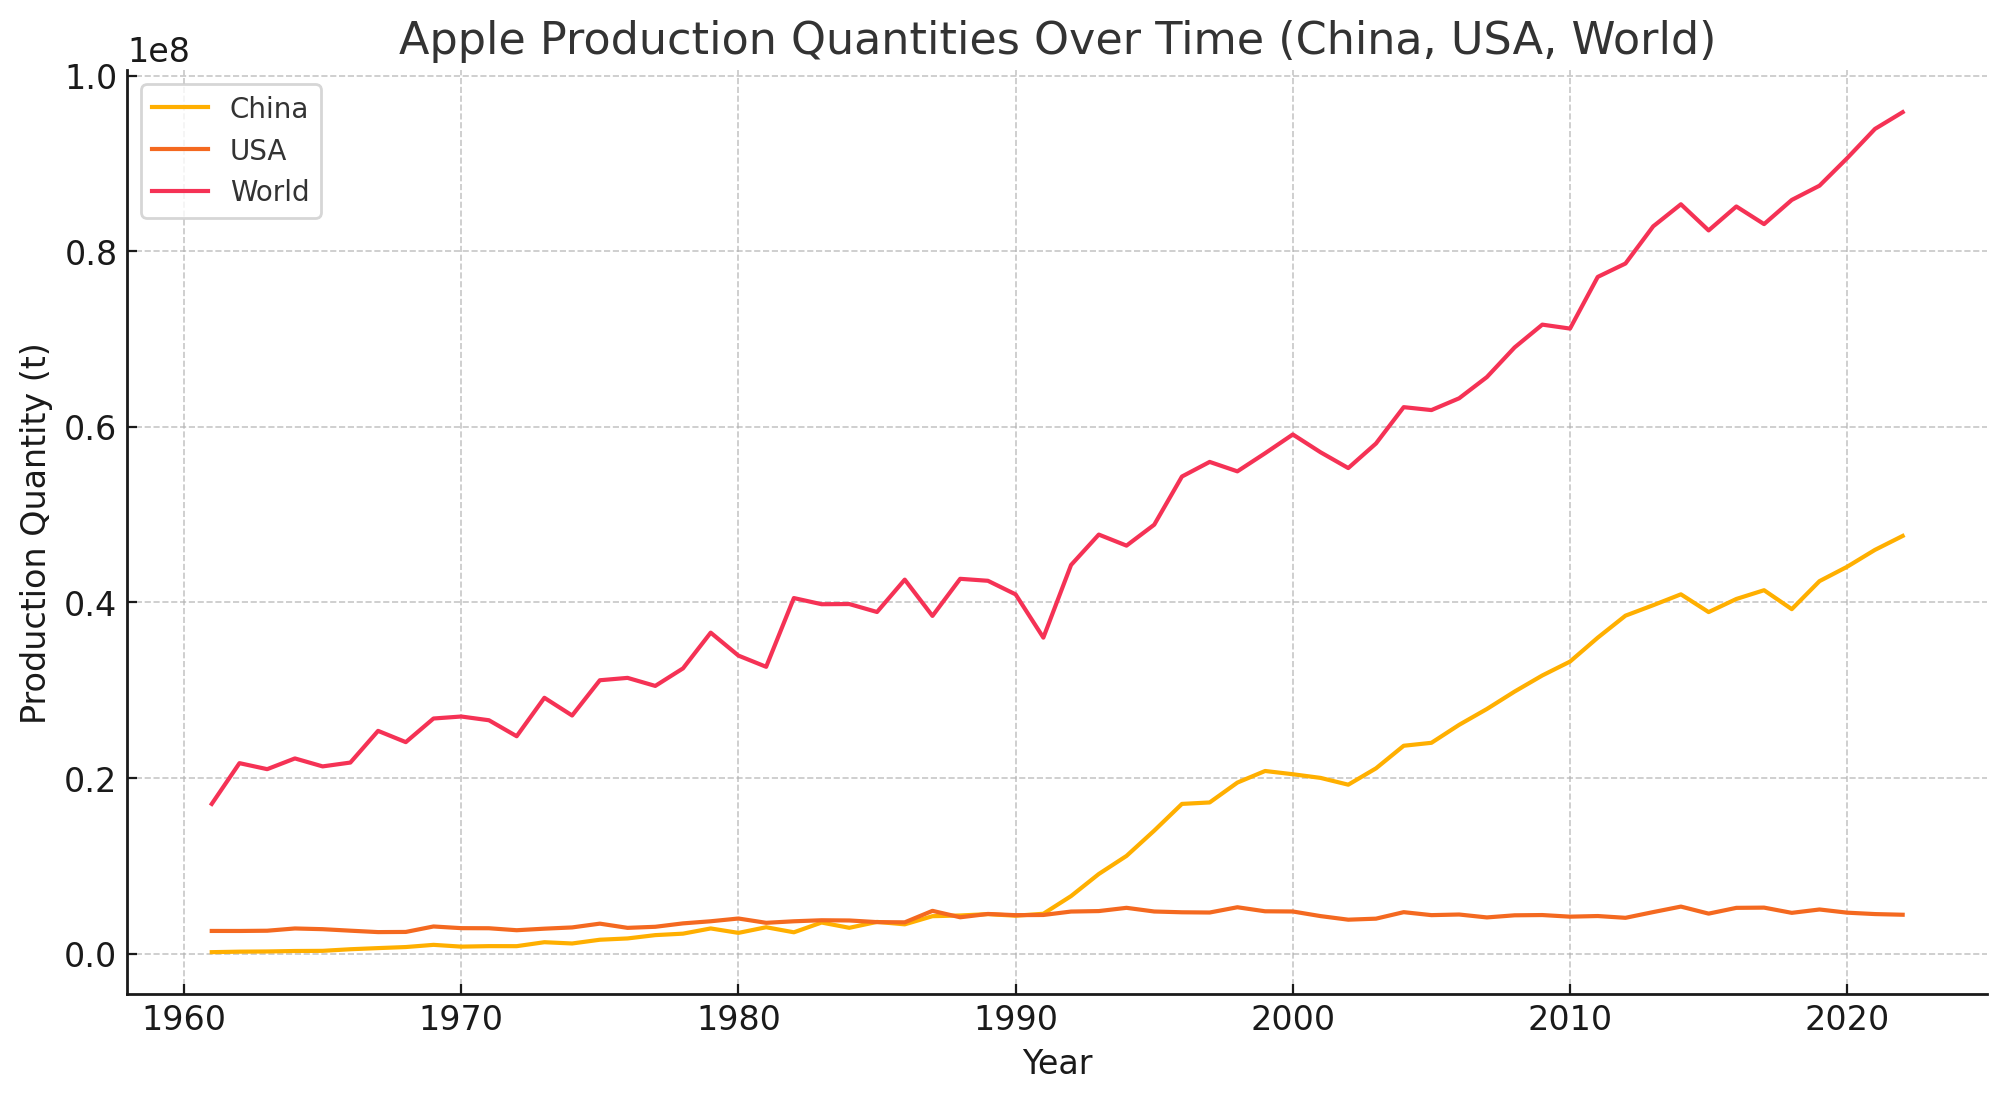
\includegraphics[width=\linewidth]{figures/production_China_US_world.png}
    \label{fig: production quantity}
    \text{Source: The Food and Agriculture Organization Statistical Database (FAOSTAT)}
\end{figure}

The rapid development of the apple industry over the past few decades in China has resulted in a dramatic increase in farmers’ incomes in low-income regions of the country. Since the Reform and Opening-up policy, apples have been at the forefront of market-oriented reforms. It was also among the first batch of agricultural products that China planned to fully liberalize in the 1980s. This early liberalization paved the way for more market-driven pricing and production decisions, which spurred growth and attracted investment into the sector.

In 2023, China’s apple planting area reached approximately 30 million mu, yielding close to 50 million tons, with the agricultural output value of apples exceeding 200 billion RMB for three consecutive years. Late-maturing red Fuji apples make up about 70\% of this total (National Bureau of Statistics of China, 2024). Globally, China led in both apple production and consumption in 2023, accounting for roughly 55\% of global apple production and approximately 53\% of global consumption (USDA Foreign Agricultural Service, 2024).

On the consumption side, the majority of apples in China are consumed fresh seasonally and domestically, with processed products occupying only a minimal share. According to USDA (2023), China's 2022 domestic fresh-apple consumption was over 46 million tons, while its annual production of concentrated apple juice nationwide was only roughly 0.3 million tons, utilizing about 2.1 million tons of apples—less than 5\% of China’s total apple harvest (YUNGUO Report, 2024).

\begin{table}[hpt]
    \centering
        \caption{Main-Producing-Province Planting area and Production in 2022}
    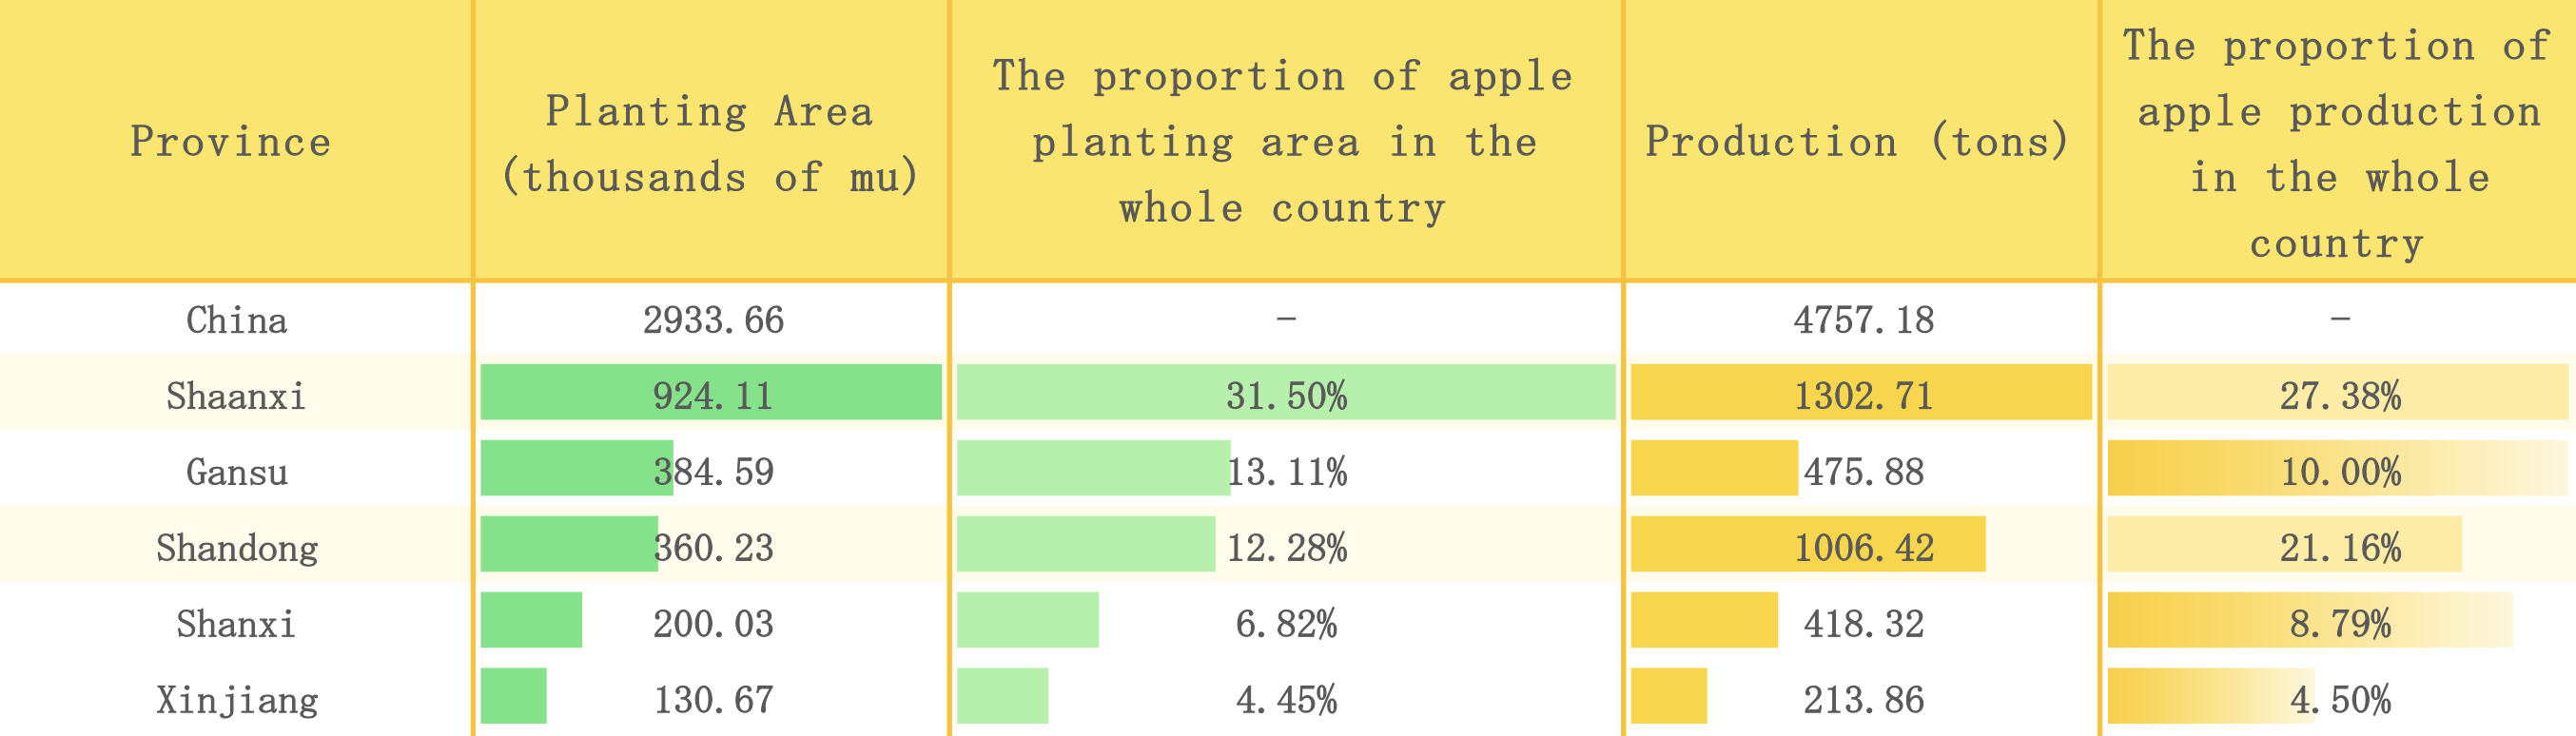
\includegraphics[width=\linewidth]{tables/production_provinces_table.png}
    \label{tab: production provinces}
\end{table}


While the national figures provide a broad overview of China’s apple industry, the regional dynamics are equally important for understanding the intricacies of this market. One province stands out as a critical player in this context—Shaanxi. The phrase "The world's apples look to China, and China's apples look to Shaanxi" captures Shaanxi Province's prominent role as the world's largest contiguous high-quality apple growing area. Recognized by the United Nations Food and Agriculture Organization as one of the “world’s best apple-producing regions,” Shaanxi’s apples are also registered as a geographical indication product in the European Union. As the leading region for both apple cultivation area and production volume in China, Shaanxi produced 13.75 million tons of apples in 2023, accounting for around 28\% of the national total.

As a representative region in China’s apple industry, Shaanxi faces significant challenges in the storage and distribution of its apples. As a storable fruit, apples have the potential to extend their market reach beyond the harvest season. But the province's storage capacity—estimated at around 5.8 million tons—is insufficient to meet the demands of local farmers and fruit traders. This shortfall points to an underdeveloped cold storage infrastructure, which affects not only the efficiency of the supply chain but also the income stability of the farmers. This gap in storage capacity is a crucial element to consider in understanding the market dynamics of Shaanxi’s apple industry, and it serves as a backdrop for our later analysis of the broader market structure of the fresh apple supply chain.



\subsubsection{Import and Export Patterns}
Despite China's leading position in apple production, the country faces significant challenges in the global apple market, particularly with regard to export volume. While Chinese apples are widely consumed domestically, their export volume remains relatively small compared to domestic consumption. The primary reason for this is not necessarily issues with quality, but rather the lack of brand awareness of Chinese apples in international markets. 

Most fruit merchants in China have not focused on developing apple export opportunities, due to limited branding, international market penetration, and a lack of export channels, logistical support, and export-friendly policies. While Chinese apples meet quality standards, the industry’s weak infrastructure for promotion and distribution has hindered growth in export markets. As shown in Figure \ref{fig: import export}, China’s exports are more variable compared to the U.S., indicating challenges in retaining international customers.

\begin{figure}[hpt]
    \centering
        \caption{Import and Export Quantities for China and USA from 1961 to 2022}
    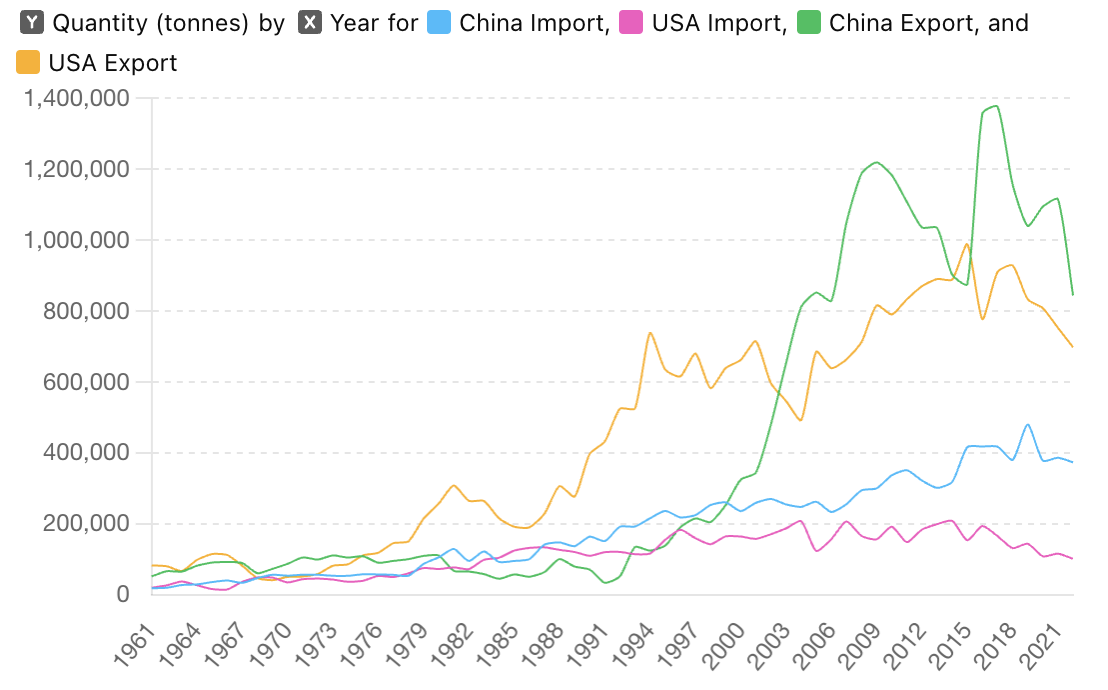
\includegraphics[width=\linewidth]{figures/import_export.png}
    \label{fig: import export}
    \text{Source: The Food and Agriculture Organization Statistical Database (FAOSTAT)}
\end{figure}

In 2023, China had a net export position in the apple trade, with exports reaching 1.07 million tons. Fresh apple exports are relatively diversified across trade partners, with key export destinations including Southeast Asian countries such as Vietnam, Indonesia, Thailand, and Bangladesh, which collectively account for over 75\% of total Chinese apple exports. Shandong province, located along the coast, contributes around 55\% of these exports. Although Shaanxi is another major apple-producing region, its inland location limits its export capacity, accounting for less than 3\% of the national total. Export activities typically peak from September to December each year.

On the other hand, as shown in Figure \ref{fig: import export}, China’s imports have remained relatively flat, highlighting its strong domestic consumption and minimal reliance on foreign apples, of 98,200 tons in 2023.  Import volumes are concentrated during the latter half of the production cycle, from April to August, when domestic inventories are low. New Zealand is the leading source of apple imports, accounting for approximately 60\% of total imports. Among China's provinces, the coastal regions of Guangdong, Shanghai, and Zhejiang make up over 95\% of the total apple imports, and relatively rich urban residents mainly consume these imported apples.





    
\subsection{Supply Chain Dynamics}
China’s fresh apple supply chain is characterized by a highly fragmented structure, seasonal supply-demand imbalances, and limited cold chain logistics, all of which restrict supply chain efficiency and contribute to significant price volatility, ultimately impacting the industry’s development.

The apple-growing segment combines regional concentration with dispersed production patterns. Key regions like Shaanxi and Shandong provinces have some clusters of concentrated orchards. Still, a significant portion of apple cultivation is managed by small-scale farmers who rely on traditional practices. This uneven production and management structure often results in fluctuations in yield and apple quality, adding variability to the supply chain.

Inefficient storage presents a critical bottleneck in the midstream segment of the apple supply chain. This issue leads to an oversupply of apples during the harvest season, driving prices down, while limited off-season inventory exacerbates price volatility due to constrained supply. The midstream market is characterized by low horizontal integration, with small- and medium-sized buyers playing a pivotal role. These buyers typically purchase apples directly from farmers, conduct initial sorting and packaging, and then sell to wholesalers (aggregators) or retailers. 

Notably, demand from the food service sector, such as restaurants, is minimal compared to household consumption. While specific data on the share of fresh apple consumption attributed to the food service industry in China is scarce, insights from my 2024 interview with the China Apple Industry Association corroborate this observation.



\begin{figure}[hpt]
    \centering
        \caption{Supply Chain of Fresh Apple Industry}
    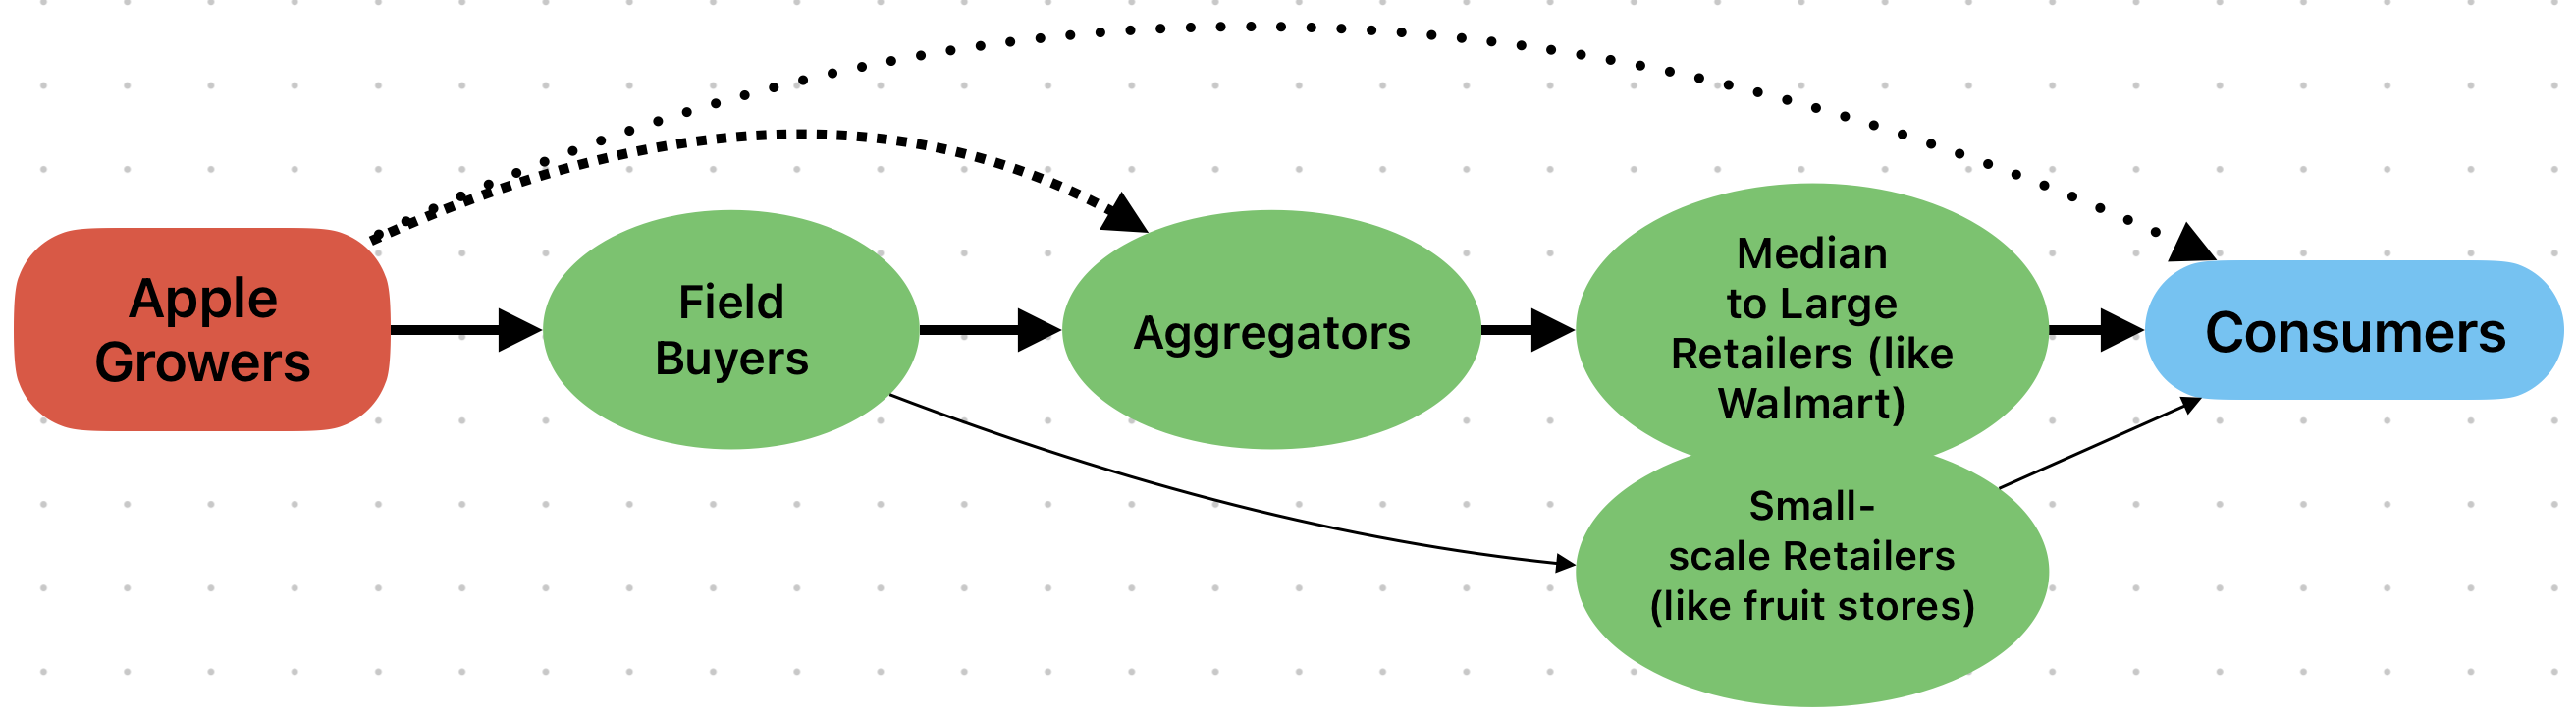
\includegraphics[width=\linewidth]{figures/Supply_Chain_flow.png}
    \label{fig: supply chain flow}
\end{figure}
The apple supply chain flows from growers to consumers through at most three layers of intermediaries, as shown in Figure \ref{fig: supply chain flow}. Each intermediary plays a distinct role, though each trader or firm may shift between roles based on timing, pricing, and market conditions. I categorize these intermediaries into kinds and define them as follows:

\begin{itemize}
    \item \textbf{Field Buyers}: These are small-scale traders who purchase apples directly from growers. Field Buyers act as the first point of aggregation, sourcing apples from orchards.
    
    \item \textbf{Aggregators/Wholesalers}: These intermediaries, often comprising larger wholesalers or processors, purchase apples from Field Buyers. Aggregators play a crucial role in consolidating apples from various sources and may add value through sorting, packaging, and broader distribution. Depending on the timing and market price, larger traders or wholesalers may also procure directly from growers, temporarily functioning as Field Buyers.
    
    \item \textbf{Retailers}: The final link in the supply chain, retailers acquire apples from Aggregators (or occasionally from Field Buyers) and sell them directly to consumers. Retailers range from major supermarkets, like Walmart and Carrefour, to smaller local stores, making apples accessible to the end consumers.
\end{itemize}

While these intermediary roles are generally stable, a trader or firm may switch between them based on circumstances---for example, a wholesaler may act as a Field Buyer during certain periods of the crop year if it offers a cost advantage. This adaptability allows the fresh apple supply chain to respond flexibly to changing market dynamics and crop cycles.




\subsubsection{Leaving the Orchard: Marketing Choices of Apple Growers}
This section addresses how apple growers sell their produce and make inter-temporal marketing decisions. First of all, the marketing timeline of primary growers is as follows: 

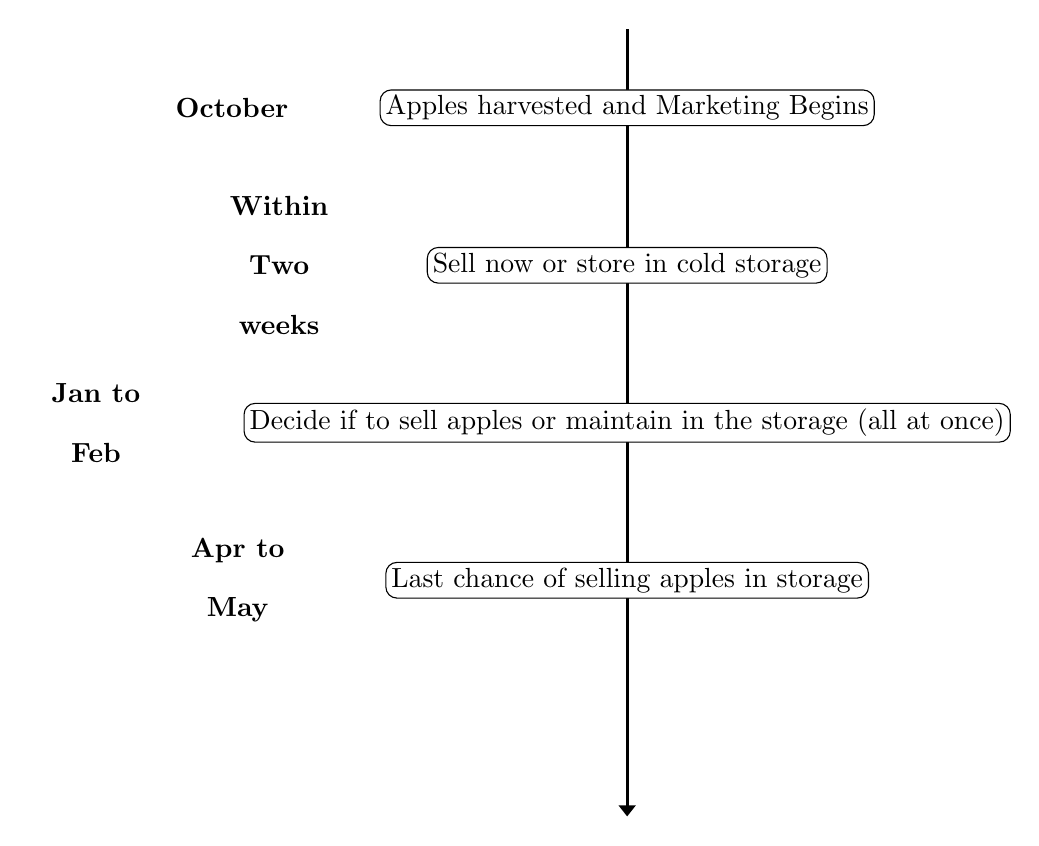
\begin{tikzpicture}[
  timeline/.style={line width=1pt, draw=black, -{Triangle[length=4pt, width=6pt]}},
  event/.style={draw, fill=white, rounded corners, inner sep=2pt},
  year/.style={text width=1.5cm, align=center, font=\bfseries}
  ]

  % Vertical Timeline (extended to handle more events)
  \draw[timeline] (0,0) -- (0,-10);

  % Events
  \node[event] (event1) at (0,-1) {Apples harvested and Marketing Begins};
  \node[event] (event2) at (0,-3) {Sell now or store in cold storage};
  \node[event] (event3) at (0,-5) {Decide if to sell apples or maintain in the storage (all at once)};
  \node[event] (event4) at (0,-7) {Last chance of selling apples in storage};

  % Years
  \node[year, left=of event1] {October};
  \node[year, left=of event2] {Within Two weeks};
  \node[year, left=of event3] {Jan to Feb};
  \node[year, left=of event4] {Apr to May};


\end{tikzpicture}


Farmers harvest their apples each year in mid to late October. Following harvest, they have a narrow window of two to three weeks to make their first decision: either sell or store the apples. There are two main ways they sell their produce:

\begin{enumerate}
    \item \textbf{Contract Sales to Large-scale Field Buyers or Aggregators}: Many farmers prefer to sign contracts with larger merchants, as these agreements offer more security. Smaller merchants are often less reliable and can easily break contracts, making farmers hesitant to work with them.
    \item \textbf{Direct Negotiation with Field Buyers}: In some cases, smaller merchants visit the village during harvest time, assess the apples, and negotiate directly with the farmers to purchase the fruit.
\end{enumerate}

This initial trading period lasts roughly two weeks. If farmers are unable to sell or choose not to sell their apples during this time, they must store them in cold storage and wait for another opportunity to sell.

While farmers can sell their apples at any time once they are in cold storage, there are two main marketing windows when they typically sell:

\begin{itemize}
    \item \textbf{The First Window}: Around January and February, coinciding with the Chinese Spring Festival. If farmers believe this is the highest price they can get, they will sell their apples at this time.
    \item \textbf{The Second Window}: If they hold onto their apples longer, the next opportunity to sell usually arises between late March and early May, around Labor Day.
\end{itemize}

Traditionally, apple growers sell their entire harvest at once when they encounter favorable pricing rather than gradually selling over time, even if prices fluctuate. This behavior is shaped by market dynamics and a preference for one-time cash inflow.

Two primary marketing channels discussed above dominate the initial stage of apple trade in China, but a small number of growers are beginning to explore direct-to-consumer sales through innovative methods. Leveraging platforms like WeChat and TikTok, these farmers are adopting multi-period smoothing sales strategies. While e-commerce currently represents only a negligible share of total sales, it offers significant advantages. This approach not only reduces information asymmetry but also allows farmers to gain a more comprehensive understanding of the supply chain, enabling them to make more informed and efficient decisions.


Moreover, most apple growers in China do not have fixed trading partners. While they may be familiar with some traders, these relationships lack strong binding ties. Farmers in the fieldwork site exhibited a strong preference for large-scale traders. These giant merchants offer greater stability and credibility, as they are perceived to have lower market failure rates compared to smaller traders. When farm-gate price differences are marginal—typically within 0.2 RMB/kg—farmers tend to favor large traders, prioritizing reliability and security over minor price advantages.




\subsubsection{Connecting the Ends: Distributing Channels of Intermediaries}
As shown in Figure \ref{fig: supply chain flow}, field buyers play a critical role in the apple supply chain, distributing apples either to aggregators or directly to small fruit shops. They operate using three main strategies, which are representative of their diverse roles:

\begin{enumerate}
    \item \textbf{"Immediate In-n-Out" Buyers}: These buyers operate on demand-driven purchases from downstream agents. They procure apples directly from farmers and immediately transport them to downstream agents without any storage, aligning their operations with real-time demand.

    \item \textbf{"Arbitrage Sellers"}: Similar to aggregators, these buyers focus on leveraging inter-temporal price differences. They typically make a single bulk purchase, store the apples in cold storage (either their own or that of larger traders), and sell them later when prices are higher.

    \item \textbf{"Cooperative Agents"}: These buyers are also apple growers who leverage their strong local social networks and access to village-level information. They typically purchase smaller quantities from local farmers and resell them to large-scale traders, acting as intermediaries.
\end{enumerate}

Aggregators, on the other hand, often establish long-term contracts with large-scale retailers such as Walmart and Carrefour, ensuring stable supply relationships. For example, in Yanchang County, the largest aggregator, \textit{China Agricultural Products Group Ltd (Yanchang branch)}, is a key supplier of fresh apples to \textit{WUMART Stores, Inc.}, which operates over 100 grocery stores in Beijing. Despite their direct procurement efforts during the peak trading season, the fragmented nature of apple production in China forces aggregators to rely heavily on field buyers for their supply.

Meanwhile, small- to medium-sized retailers, such as street-side fruit shops in urban areas, often bypass aggregators and source directly from field buyers. This approach allows them to secure lower procurement costs or obtain unique, high-quality apples that distinguish their offerings from those of large-scale retailers, thereby carving out their own market niche.

While international demand accounts for only a small portion of the total fresh apple consumption in China, exporters often maintain greater vertical integration compared to purely domestic players. Companies like \textit{Yantai North Andre Juice Co.} and \textit{Shaanxi Fruit Industry Group Co.} employ dedicated procurement teams to ensure their apples meet international quality standards. These teams establish long-term relationships with farmers, offering technical and financial support to achieve product consistency.

China’s apple exports are primarily destined for Southeast Asian countries, where consumers often prefer smaller-sized apples rather than the widely cultivated Red Fuji variety. To meet this demand, exporters must develop their own supply sources instead of relying on existing orchards and intermediaries.




\subsubsection{Middlemen Scale and Supply Chain Roles}
The scale of a buyer is closely tied to its role in the supply chain. Smaller buyers typically have less capital, lower purchasing volumes, limited storage capacity, and reduced risk tolerance. However, their trading strategies tend to be more flexible. As a result, small buyers rarely sign long-term supply contracts with downstream clients. During the initial trading period following the harvest, they often wait for large buyers to set the market price before making their moves.

Intuitively, one might question why small buyers persist on a large scale if they seem to lag behind large buyers in every aspect. The key lies in their role as field buyers within the supply chain. Their greatest value is their ability to reach fragmented and scattered micro-scale apple producers in a way that is not as visible or accessible to larger buyers. This effectively extends the supply chain extensively. At the same time, small buyers often exploit the information asymmetry inherent in these small-scale trading relationships to generate excess margins.

In my fieldwork region, Yanchang County, there are four large-scale fresh apple traders, primarily serving as aggregators. With large cold storage facilities (over 5,000 tons), these traders purchase fresh apples from farmers exclusively during the initial trading period after the harvest (mid-to-late October), fulfilling their annual procurement needs in one go. In contrast, hundreds of small-scale buyers emerge in the county each year, sourcing apples from farmers over a dispersed period of six to eight months after the harvest.

For apple farmers, becoming a supplier to large-scale traders is challenging due to their stringent requirements, which often include larger orchard sizes, higher fruit quality, and a proven track record of honoring contracts. Unfortunately, given the constraints of production conditions and education levels in developing regions like northern Shaanxi, China, most farmers in these areas are left with no choice but to sell their apples to small-scale buyers.

From the perspective of end consumers, demand is diverse and virtually limitless. Thus, small-scale retailers can always find niches, which have not been satisfied by supermarkets, to thrive in—whether through geographical market segmentation, offering a variety of apple qualities, or aligning with niche brands.

In summary, in the fresh apple industry in China, small-scale buyers typically occupy the two ends of the intermediary spectrum illustrated in Figure \ref{fig: supply chain flow}: they exist as field buyers and small-scale retailers. Their foundation lies in the diverse and dispersed nature of suppliers and consumers.




\subsubsection{Dynamics of Local and non-local Traders \label{Section: intro of Local and non-local traders}}
Similar to many other agricultural commodity markets, such as California's tomato industry \citep{hamilton2024spatial}, China's fresh-apple procurement markets are often localized at the county level. These markets are characterized by a limited number of buyers and the potential for hold-up due to costly cross-county transportation and the perishability of apples. Consequently, most intermediaries fall into two distinct groups: ``local traders'' and ``non-local traders.''  

``Local traders'' refer to merchants based in the same county, whose primary trading activities are also concentrated within the county. In contrast, ``non-local traders'' are merchants from other regions who specifically travel to the county to purchase apples.  

Local fruit traders are mostly small-scale operations. They typically earn a margin by reselling to non-local traders rather than directly supplying downstream markets themselves. According to a local trader in Yanchang County, Wenkui Liu, \say{only a small fraction of them handle downstream distribution on their own. In contrast, non-local traders who come to purchase fruit are usually more established and often have their own dedicated apple distribution channels.}

Local traders typically have a deeper understanding of local apple production, knowing exactly which villages or even households consistently supply high-quality and reliable products. They are also well-acquainted with the distribution of cold storage facilities, government regulations, and other county-specific information critical to the apple supply chain upstream. Therefore, in economically developed regions with high-quality apple production, local traders are often numerous and dominant, unwilling to relinquish their control over the upstream supply chain to outsiders. non-local traders entering these regions must compete with local traders at an intrinsic disadvantage. Therefore, most non-local traders resort to ``subcontracting'' local traders to source apples on their behalf, forfeiting part of their profit margins.  

Conversely, in economically less developed areas, non-local traders tend to have a higher market share. This is partly because local traders with a solid understanding of the market often migrate to high-quality production areas in search of better opportunities. Additionally, non-local traders frequently serve more diverse purchasing needs, such as supplying lower-quality apples to juice factories or taking advantage of weaker relational considerations and negotiation costs in less developed areas, where bargaining power may be more favorable to buyers.  

Moreover, some traders purchase apples from lower-quality production areas and then repackage or store them in high-quality regions, thereby disguising their origin to command higher prices. For instance, apples from Yantai in Shandong Province have established a strong reputation nationwide. In recent years, however, many ``non-local'' apples have been stored in Yantai’s cold storage facilities, only to be sold later under the Yantai label at premium prices. Downstream buyers often find it difficult to distinguish these apples from the genuine local produce, leading to significant brand and regional price markups to those non-local traders.


\subsection{Roles of Storage \label{Section: role of Storage}}
In China's fresh apple industry, storage serves multiple roles across different stages in the fresh apple supply chain, stabilizing inter-temporal supply, maintaining apple quality, and managing market dynamics across seasons. As a storable agricultural product, the shelf life of apples can be significantly extended by using cold storage. Apples can be preserved for several months, or even up to a year, in a cold storage environment at around 0°C and 85\%-90\% humidity, whereas at room temperature, they can only last for a few weeks.

The use of cold storage facilities is highly diversified and fragmented, with the entire supply chain relying on cold storage, and the distribution ratio changing each year. From the perspective of market efficiency theory, most apples awaiting sale should ideally be stored in cold storage with the lowest unit cost, which is typically in the ultra-large cold storage facilities owned by major fruit traders. However, due to various transaction frictions and information asymmetry, large traders' cold storage facilities tend to hold a complex inventory, with around 50\% of the stock on average consisting of apples owned by the storage owners themselves. The remaining stock is mainly stored on behalf of various small traders and local, experienced apple growers.

At the farm level, after picking, farmers make initial decisions about selling vs. storing. Storage enables them to delay sales until market conditions improve, allowing them to wait for higher prices in off-peak seasons, which can improve their overall income stability. Additionally, storage facilities provide smallholders with the flexibility to sort and grade apples at their own pace, reducing post-harvest losses and maintaining quality. However, their storage options are limited and often depend on available infrastructure nearby. Despite a few forward-thinking farmers building their own small cold storage facilities, the overall adoption rate of cold storage among apple growers remains low. With government subsidies, many villages have built medium-sized cold storage facilities with capacities of several hundred tons, collectively owned. However, this leads to a low individual harvest-to-storage-volume (HSV) ratio, mainly because of the high storage cost. This is because the use of such collectively-owned cold storage requires multiple farmers to coordinate their decisions after harvest, which often is very hard.

Intermediaries purchase apples from farmers, either for immediate resale or for storage. For them, storage serves as a key function for aggregating apples from different growers. This aggregation enables sorting, grading, and packing before the apples move to larger markets or processors. It also provides intermediaries with greater bargaining power by controlling the flow of apples into the market, allowing them to release apples gradually and manage supply to influence prices. This is particularly important in an oligopsonistic market structure, where a small number of buyers dominate the market. Furthermore, storage ensures quality assurance for downstream buyers, such as wholesalers and retailers, by maintaining apples in optimal conditions, ensuring they meet high-quality standards, especially for urban markets or export.

Retailers, especially in urban areas, rarely own or rent storage facilities specifically for fresh apples but usually cooperate with large-scale intermediaries, signing long-term supply contracts and leaving apples in the suppliers' facilities. Once there is a potential shortage of apples on the shelves, apples can be replenished from the supplier's cold storage at any time. This practice supports retailers' stock management, helping retailers avoid overstocking while still ensuring that apples are available to customers.

Finally, for apples intended for export, storage is essential for maintaining quality during transit. Export-ready apples, especially those shipped long distances to markets in Southeast Asia and other regions, often require controlled atmosphere storage to preserve freshness, appearance, and taste. This storage minimizes spoilage risks during shipping and helps meet the stringent quality requirements of international markets.




\subsubsection{Storage Pricing Structure: Based on Quantity, Not Duration} 
Cold storage fees for fresh apples are typically based on quantity rather than duration, which may seem counter-intuitive. This pricing structure stems from the fact that apple harvesting occurs within a narrow window (mid-October to mid-November), creating a surge in storage demand during that period. Additionally, apples can only be stored for up to a year, requiring them to be sold two or three months before the next harvest. This arrangement provides cold-storage users with a longer marketing window without any additional cost, reducing the pressure to accept lower prices from downstream buyers and giving them more flexibility in timing their sales.

\subsubsection{Shortage and Inefficient Allocation in Cold Storage Infrastructure} 
In 2022, China’s total apple storage capacity exceeded 20 million tons, with mechanical cold storage accounting for approximately 70\%, simpler storage methods making up around 25\%, and high-end controlled atmosphere storage comprising about 5\%. Over the past decade, advancements in technologies such as intelligent sorting, rapid pre-cooling, 1-MCP (1-methylcyclopropene) treatment, near-freezing point storage, and specialized preservation bags have significantly improved the commercial quality of apples and substantially reduced post-harvest loss rates.

However, given the large scale of domestic apple production and the fact that many production areas are situated in underdeveloped and poorer regions, there is a notable shortage and inefficient allocation of cold storage infrastructure. In more economically developed provinces and counties, such as Shandong, there are more cold storage facilities with larger capacities. For instance, in 2022, Shandong's total cold storage capacity was around 5.4 million tons, with actual storage usage remaining stable at approximately 4.8 million tons in recent years. The ratio of apples stored by farmers compared to those stored by traders is approximately 70\% to 30\%. On the other hand, in remote regions like northern Shaanxi and Xinjiang, the situation is starkly different: cold storage facilities are limited, and the storage needs of farmers and small-scale traders cannot be fully met. As a result, the proportion of apples in storage fluctuates significantly each year, driven largely by market conditions and sentiment.

At the micro-level, in my fieldwork area, Yanchang County, the prevalence of small, self-built cold storage units among farmers is less than 5\%. Most apple growers are forced to sell their apples immediately upon harvest or rent cold storage space from facility owners, typically traders. The cold storage capacity in this county is fully utilized each year, meaning that overall storage capacity falls short of the demand.
    







\subsection{Apple Futures Market: The World's Only Fresh-Fruit futures}
Launched on the Zhengzhou Commodity Exchange (ZCE) in 2017, China’s fresh apple futures market is the world’s only futures market dedicated to fresh fruits. As China leads global apple production, accounting for over half of the world’s supply, this market was designed to address the apple industry’s high price volatility and provide much-needed price risk management tools for farmers, traders, and buyers.

Uniquely focused on fresh rather than processed apples, this futures market stands out from traditional agricultural futures, which typically center on commodities that are shelf-stable and have relatively low storage requirements. The contract is based on the widely consumed Red Fuji variety. Contracts require high-quality apples that meet rigorous standards for both domestic and export markets, ensuring that delivered products align with consumer expectations.

The apple futures market serves as a vital bridge between various industry players, including growers, traders, processors, and exporters. By establishing a transparent pricing mechanism, it helps participants manage price risks effectively, especially in a market where prices can vary widely due to seasonal cycles, regional production differences, and changing demand. For example, in years with poor harvests, prices can rise as much as 20\%, while bumper years can see sharp price drops. Futures contracts allow growers and traders to lock in prices in advance, protecting against such fluctuations.

However, the perishable nature of apples poses logistical challenges. Maintaining quality during storage is critical for contract fulfillment, as fluctuations in storage conditions can affect both quality and price. Most apple futures contracts are executed from October through February to align with peak harvest periods, ensuring optimal product quality and reducing the need for long-term storage. 

Participation in the futures market, though, remains challenging for smaller farmers. Limited access to capital and a lack of trading knowledge can hinder direct engagement. 


%----------------------------------------------------------------%
%----------------------------------------------------------------%

\newpage
\section{Upstream Buyer Power, Market Structure, and Competition \label{Section: market structure}}

Research in the industrial organization (IO) of agricultural markets—both in developing and developed economies—has traditionally focused on the exercise of monopoly power in the sale of farm inputs, processed foods, and food retailing \citep{macdonald2024introduction}. However, significant attention has also been directed toward understanding monopsony and oligopsony power in agricultural markets, where buyers wield considerable influence over pricing and farmers' production and post-harvest decisions \citep{kopp2021farmers, zavala2022unfair}.

The structure of China's fresh apple supply chain provides a particularly compelling case for exploring these dynamics. The combination of the industry's distinctive characteristics and its critical role in rural development makes it a fertile ground for bridging insights from development economics and industrial organization research \citep{bellemare2022agricultural}. China's fresh apple industry, which accounts for over half of global production, is renowned for its impact on poverty alleviation in some of the country’s least-developed regions. The distributional impacts of market power exerted by intermediaries often outweigh its efficiency effects \citep{sexton2013market}.

This leads to a central question: Who really profits from China’s apples?

\begin{quote}
    In 2020, an informal investigation by China’s Ministry of Agriculture traced the journey of apples from orchards in Shaanxi to retail shelves in Shanghai—a 3,400-kilometer journey that saw prices increase more than fivefold. Initially, a field buyer purchased 3 kilograms of apples directly from farmers for 10 RMB. After transportation to Jiaxing and accounting for logistics costs, 10 RMB bought only 2 kilograms. Following additional sorting and distribution through wholesale markets, the same amount fetched just 1 kilogram. Finally, in Shanghai supermarkets, 10 RMB was exchanged for a mere 0.5 kilograms.
\end{quote}

At every stage of this apple's journey, the farmer’s share diminishes, implying the possibility of upstream buyer power. This example underscores critical questions about the distribution of value along the supply chain and the competitive forces—or lack thereof—that shape outcomes for stakeholders.

Based on my fieldwork in 2023 and 2024, the apple market in Northwest China operates as a buyer's market. Apple farmers (sellers) function in a near-competitive market, while intermediaries (buyers) often exhibit collusion or even oligopsonistic behavior. While some argue that farmers could secure better prices through cooperatives, most local cooperatives are too small in scale compared to buyers' procurement volumes and face significant competition among themselves. Additionally, cooperatives are loosely organized, leaving most farmers to sell individually. Buyer competition, however, is closely tied to downstream demand. During periods of low demand, field buyers rarely compete, but in times of strong demand, intensified competition for market share drives up farm-gate prices.

This section depicts the market structure and competition within the upstream segment of China's fresh apple supply chain, with a particular focus on buyer power. The analysis draws on descriptive micro-level evidence gathered during my fieldwork in Yanchang County, Shaanxi Province, China.



\subsection{Collusive Behavior and Competition Among Local Traders}

In Yanchang County, local field buyers exhibit significant collusive behavior, forming numerous field-buyer cartels. While these small cartels are multiple at the county level, their prevalence decreases at more localized levels, such as towns or villages, where their numbers typically range from one to three. These structures effectively create market conditions ranging from monopsony to oligopsony.

Each field-buyer cartel usually operates as a unified entity, coordinating its procurement activities and deliberating strategies prior to engaging in apple purchasing. These cartels utilize information-sharing mechanisms, such as WeChat groups, to exchange real-time farm-gate price data and maintain price discipline by avoiding undercutting. Furthermore, they strategically plan procurement tactics to influence market outcomes. For instance, Buyer A described the coordinated practices as follows:

\begin{quote}
\say{My associates and I prearrange strategies to manage farmers' price expectations. On the first day, I might visit a village and offer a certain price without closing any deals. The next day, my colleague followed up with a deliberately lower price. Concerned about losing a buyer, farmers often agree to sell. This enables us to acquire apples at reduced prices.}
\end{quote}

The high degree of coordination among members within a cartel reflects their strategic alignment in establishing an oligopsonistic bargaining position. According to another Buyer B:

\begin{quote}
\say{We avoid competition during the sourcing stage because our downstream distribution channels are almost entirely distinct from one another.}
\end{quote}

Despite the internal cohesion of individual cartels, inter-cartel competition is presented. This inter-cartel rivalry is primarily driven by concerns over sourcing higher-quality apples and safeguarding supply sources. Yinfang Lei, the manager of \textit{Shaanxi ZhongGuo Ltd.}, a local aggregator, remarked:

\begin{quote}
\say{The competition between field-buyer cartels is intense. They are wary of other cartels capturing higher-quality apples or encroaching on their supply bases, which could undermine their market position. Consequently, cartels are generally unwilling to collaborate with one another.}
\end{quote}

The behavior of these cartels highlights classic dynamics in the field of industrial organization, where coordination within a group aims to enhance buyer power, while inter-group competition undermines broader collusion. The duality of cooperative and competitive forces underscores the complex strategic interactions within localized agricultural markets.



\subsection{Market Territories of Buyers}
The existence of market territories among buyers in Yanchang County is a subject of debate.

Although field-buyer cartels generally do not cooperate, traders within a given cartel coordinate their procurement areas, establishing informal market territories to avoid internal conflicts. For instance, Buyer A in LeiJiaTan Town noted: 

\begin{quote}
\say{A market territory does exist. I will not step into a village if another member of my group has already contacted it during the same crop year. This happens in about two-thirds of cases now.}
\end{quote}

As illustrated in Figure \ref{fig: Market Territory}, within Cartel 1, four traders procure apples separately from Villages 1, 3, 4, and 5 without interfering with each other. These market territories are not formally delineated but are instead based on verbal agreements. Each cartel redefines its internal market territories annually, ensuring flexibility to adapt to shifting procurement conditions. This yearly restructuring allows cartels to exert short-term buyer power, where future considerations are relatively less significant \citep{sexton2013market}. Enforcement of these informal agreements relies on implicit relational costs rather than explicit penalties, where the cost of defection is the potential loss of trust and cooperation within the group.

\begin{figure}[hpt]
    \centering
        \caption{Market Territory Allocation Among and Within Cartels in Yanchang County}
    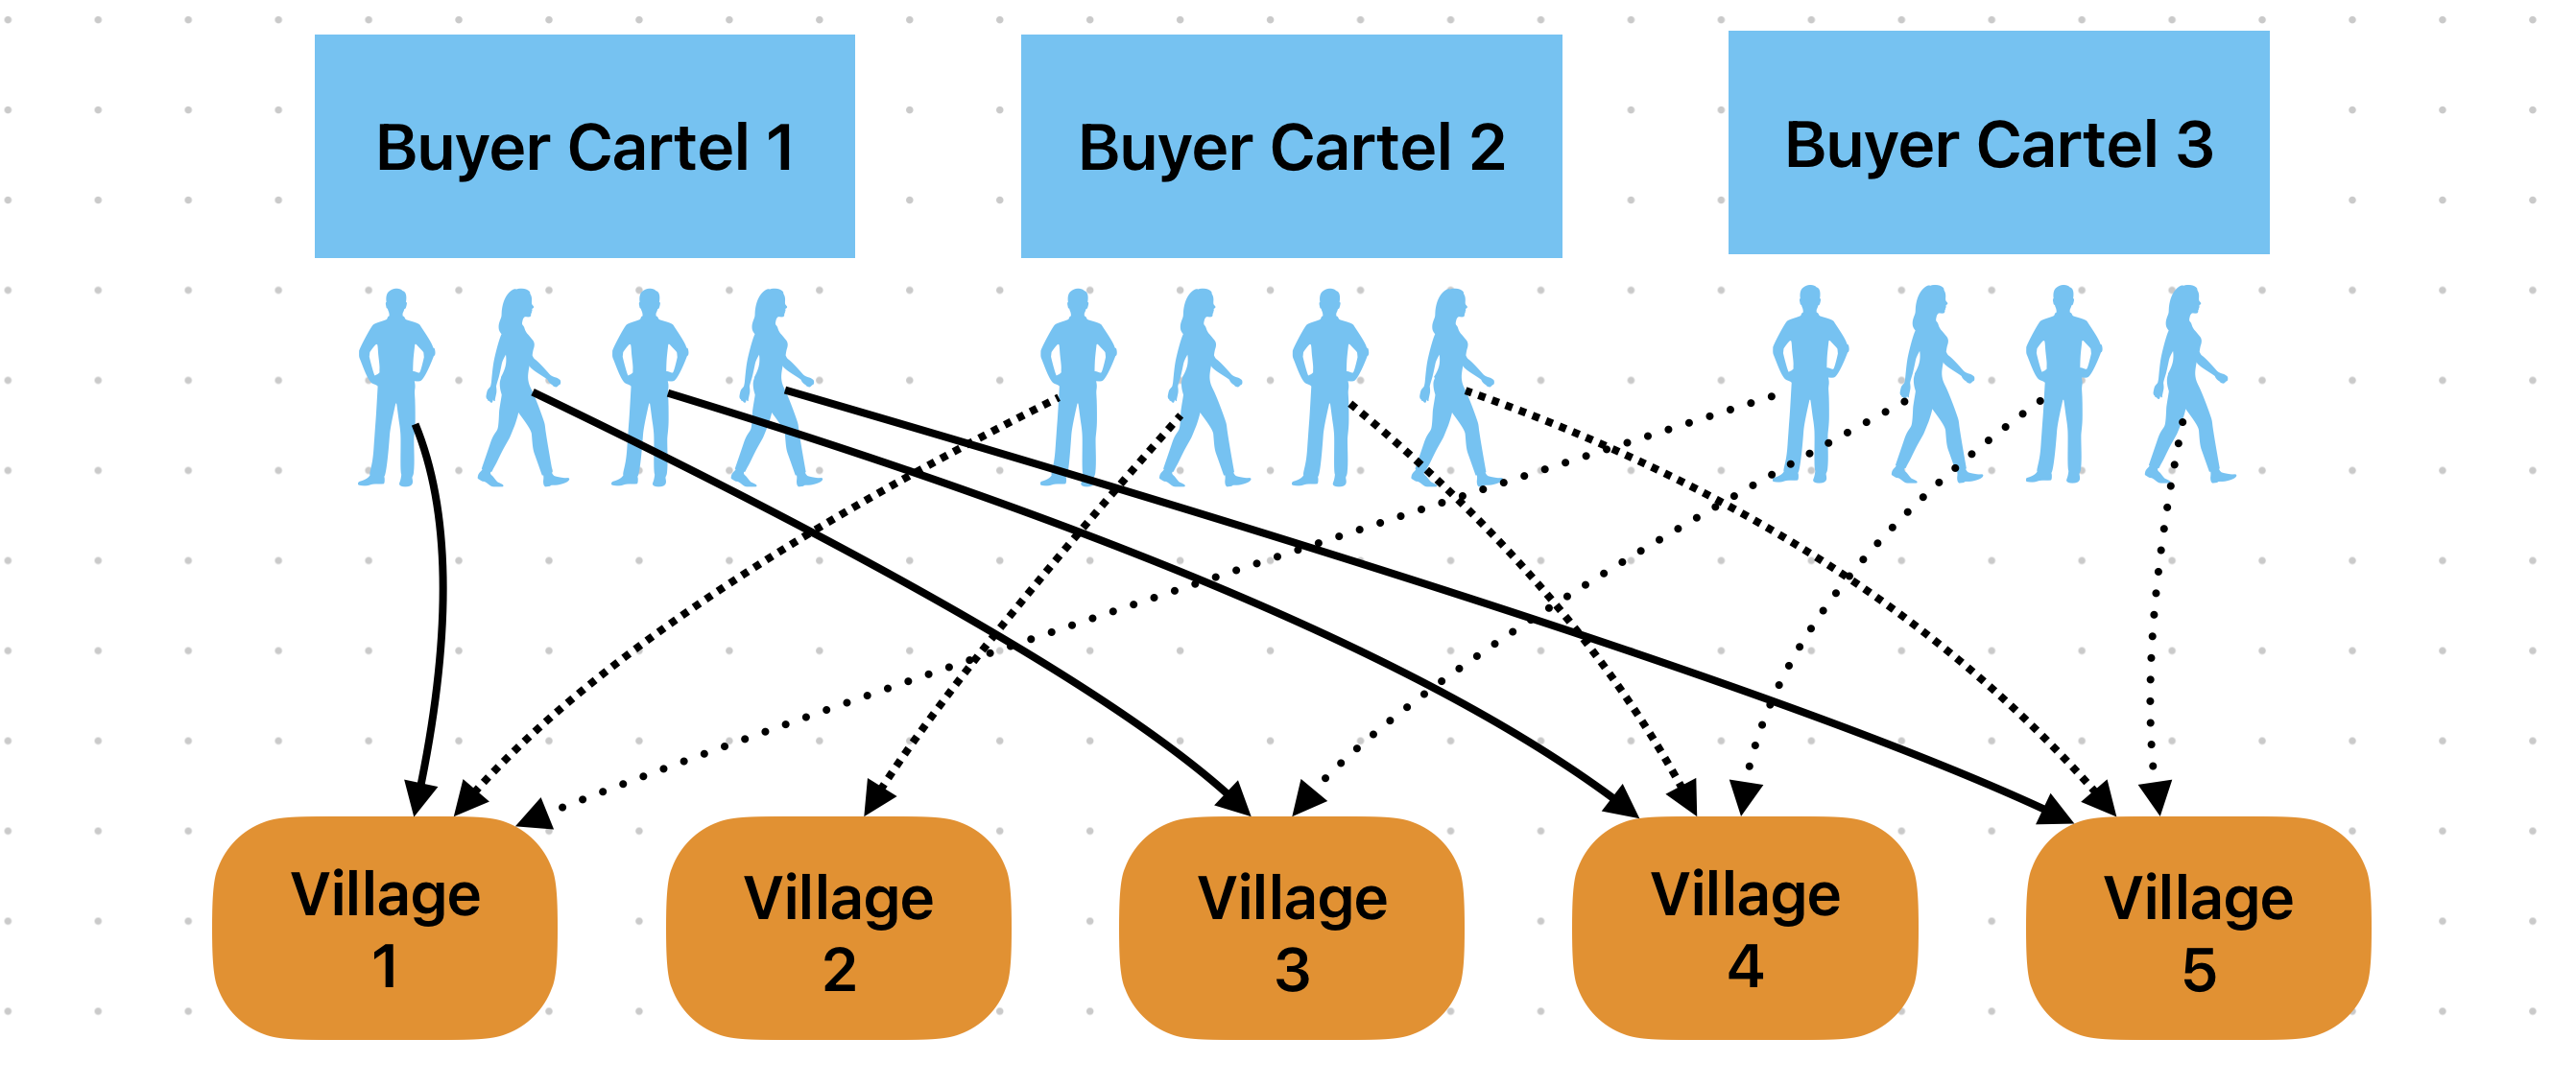
\includegraphics[width=\linewidth]{figures/Market_Territory.png}
    \label{fig: Market Territory}
\end{figure}

In contrast, there are no clear boundaries between the territories of competing cartels. Overlaps in procurement areas frequently arise, especially when multiple cartels target the same high-yield, high-quality orchards. As shown in Figure \ref{fig: Market Territory}, while Cartel 1 members respect internal market boundaries, Villages 1, 4, and 5—which produce superior-quality apples in large quantities—attract traders from all three cartels, creating an effective oligopsony. Conversely, in Village 2, only traders from Cartel 2, which is geographically closest, procure apples, resulting in a localized monopsony.

This overlapping of procurement territories among cartels demonstrates a dual dynamic: internal coordination fosters oligopsonistic market power within cartels, while external competition between cartels introduces inter-group rivalry, reducing market concentration. 



\subsection{Competition Between Local and Outside Traders}

As introduced in Section \ref{Section: intro of Local and non-local traders}, two types of apple traders operate in each county: local traders and non-local traders from outside areas.

In Yanchang County, most local traders do not manage downstream distribution themselves. Instead, they typically act as primary intermediaries (\textit{Daiban}), earning a margin by reselling apples to non-local traders or local aggregators as subcontractors. They can be categorized into:
\begin{itemize}
    \item Full Agents: Handle sourcing, sorting, and transportation, earning approximately \$0.70/kg.
    \item Assistant Agents: Focus solely on matchmaking, earning about \$0.08/kg.
\end{itemize}

Although local and non-local traders occasionally collaborate, as previously discussed, competition between them is more prominent. This competition arises because, for many non-local traders sourcing apples in Yanchang County, the additional costs associated with involving an additional local middleman often outweigh the benefits. As a result, non-local traders frequently bypass local traders by directly hiring local “information agents” to scout villages, inspect produce, and identify suitable suppliers. In many cases, non-local traders procure apples directly from farmers.

Interestingly, during the initial trading period, non-local traders often form one or more cartels to counteract local traders as well. According to a contact in Huasheng Fruit Co., a large fresh-apple exporter, \say{we, as non-local traders, commonly stay in the same hotel in the county's downtown area before heading to the villages for procurement.} These informal gatherings allow them to establish connections and organize interest groups, strengthening their collective bargaining position against local traders.






%----------------------------------------------------------------%

\subsection{The Paradox of Plenty: When More Buyers Deepen Farmer Challenges}
Is the degree of industry concentration always positively correlated with the extent of market power and negatively associated with the industry’s output level and social welfare? Recent studies, such as \cite{merel2017buyer} and \cite{crespi2012competition}, challenge this conventional wisdom, demonstrating that the relationship may not always hold.

The upstream dynamics of China's fresh apple industry demonstrate that increasing small-scale buyers in agricultural procurement markets does not always enhance competitiveness and social welfare. Instead, it could reinforce the market power of dominant buyers through intermediation and territorial segmentation, ultimately reducing farmers' bargaining power. On the other hand, wholesalers or large traders could play a pro-competitive role \citep{Belton_et_al_2024}. Fewer large buyers might better support farmers' welfare by enabling antitrust actions and fostering greater accountability in pricing practices.


\subsubsection{"More but Dispersed" or "Less but Regulated"?}
While it is a common belief among development economists that more traders in a market imply higher competitiveness, this assumption may fail in agricultural procurement markets. For instance, in scenarios where an oligopsony exists, when several large-scale dominant buyers exercise significant control, small-scale traders typically function as intermediaries rather than as true competitors. Instead of challenging the incumbent buyers' market power directly, these small-scale buyers might act as middlemen, purchasing from farmers to resell to the dominant buyers. 

In fact, a tacit agreement might even exist between the dominant large-scale buyers and these small-scale traders. Rather than acting as independent competitors, these small-scale buyers can be seen as informal extensions of the incumbents' operation, effectively functioning as outside employees or contractors. This arrangement allows the dominant buyer to maintain control over the supply chain indirectly, leveraging the small-scale traders to handle transactions with suppliers while still dictating terms and prices. Consequently, the presence of multiple traders does not necessarily dilute the incumbent buyers' influence; it may even reinforce it, thereby sustaining or worsening the oligopsonistic structure and limiting fair pricing for farmers.

\begin{figure}[hpt]
    \centering
        \caption{"More but Dispersed" vs. "Less but Regulated"}
    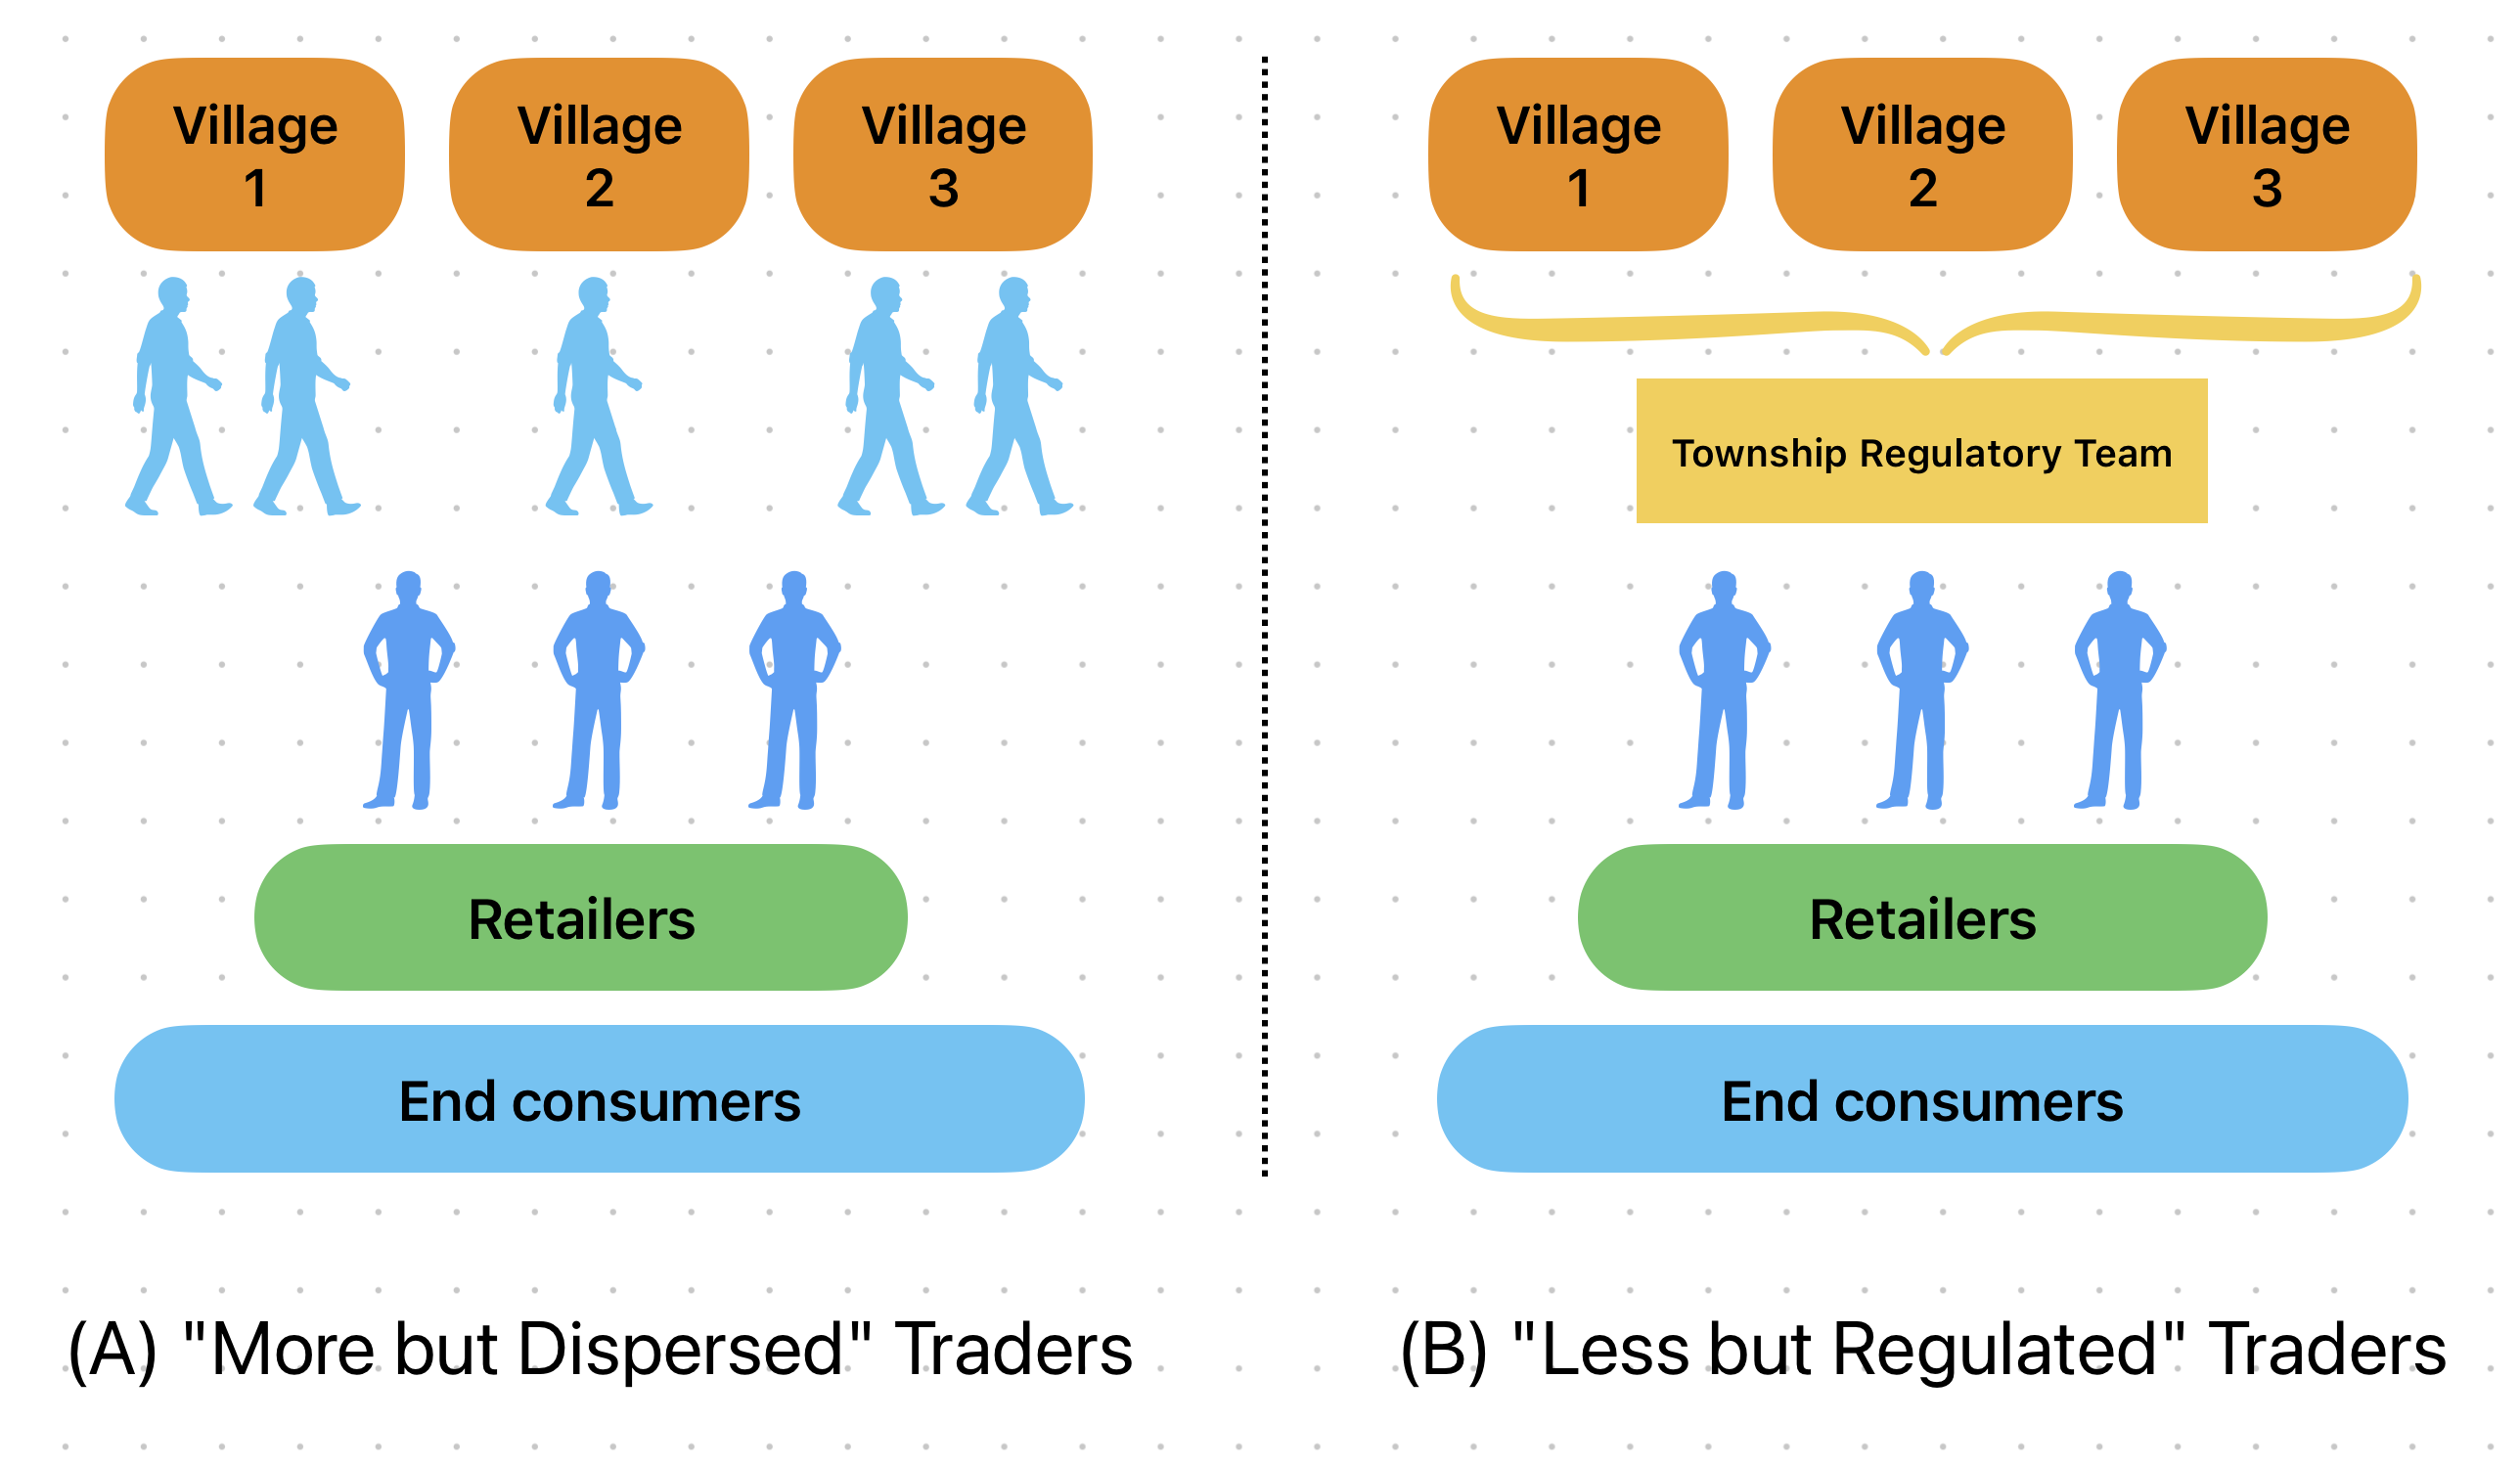
\includegraphics[width=\linewidth]{figures/more_is_less.png}
    \label{fig: more is less}
\end{figure}

In other words, as illustrated in the left panel of Figure \ref{fig: more is less}, these small-scale buyers may add another layer of intermediation, worsening both distributional fairness and market efficiency. Beyond these vertical impacts on the industry structure, an increase in entrant buyers also introduces horizontal market segmentation, often along geographic lines, which could possibly further lead to lower farm-gate prices, higher consumer prices, and significant price fluctuations across regions and over time, resulting in substantial welfare losses \citep{bergquist_McIntosh_2024}.


My fieldwork conducted during the 2023 and 2024 harvest seasons in Yanchang County revealed that over a hundred buyers traveled to various towns to procure apples each year. These buyers formed several field-buyer cartels, characterized by implicit arrangements on market territory allocation, as discussed in Figure \ref{fig: Market Territory}. As a result, farmers in each village were compelled to negotiate with a limited number of designated traders who, due to limited competition within their respective localities, could effectively suppress farm-gate prices.

Regulation at the village level has proven to be practically infeasible. While one might argue that local governments with strong leadership could function like bargaining cooperatives—negotiating collectively on behalf of farmers—this is unrealistic at the village level. The limitations are illustrated by the words of the Party Secretary of Nanpo Village during an interview conducted in the first week after the 2024 harvest season:

\begin{quote} \say{I cannot demand or prevent traders from colluding; all I can do is plead with them for a slightly higher farm-gate price for my village. Otherwise, they’ll simply leave and source apples from other villages. They have countless options elsewhere.} \end{quote}

This dynamic leaves farmers exposed, lacking both a robust regulatory framework and effective legal tools to contest the collusive practices of buyer cartels. The absence of competitive pressures and enforcement mechanisms allows buyers to continue extracting surplus from farmers, further entrenching economic vulnerabilities in rural communities.


Paradoxically, a market dominated by a few large buyers may offer better outcomes for farmers. With fewer, larger players, antitrust enforcement and collective legal actions become more practical. The right panel of Figure \ref{fig: more is less} shows that under feasible township regulation, each village effectively faces the competition among three primary buyers, instead of at most two in the left panel case. Furthermore, the reputational risks and higher visibility associated with large-scale operations can deter exploitative practices. While concentrated market power among a few buyers might initially appear detrimental to farmers, it can, in practice, enhance farmers’ bargaining leverage by enabling meaningful oversight and accountability.

Unlike other towns in Yanchang County, Angou Town exemplifies this dynamic. Thanks to the stable quality and high yield of apples across its villages, the local primary apple procurement market is dominated by three large buyers: \textit{Huasheng Fruit Co}, \textit{the Yanchang branch of the China Supply and Marketing Cooperative}, and \textit{Shaanxi Zhongguo Ltd}. These major players have effectively pushed out smaller buyers, who rarely venture into the area.

The village secretary of Huangguyuan Village in Angou Town, explained:
\begin{quote}
    \say{In Angou Town, the government helps farmers negotiate collectively with the three major buyers. Oversight of these companies is also more straightforward. First, due to their large scale and presence, they maintain physical offices locally, allowing regulators to contact them directly at any time. Second, the farmers in Angou Town are generally better educated and understand contractual obligations. They rarely undermine agreements negotiated with the major buyers for a slightly higher price from other small-scale traders}
\end{quote}
This structured approach fosters a cooperative relationship between farmers and large buyers, underpinned by government-supported negotiation and effective regulatory oversight. In Angou Town, concentrated market power appears to enable fairer pricing and greater stability for farmers, highlighting the potential benefits of a more concentrated market structure under appropriate institutional support.


This seemingly counter-intuitive phenomenon may possibly be explained by several underlying mechanisms, often requiring only one or two specific conditions. For example, as \citep{sexton2018increasing} illustrates, even in a highly concentrated procurement market, if buyers place sufficient value on the future—that is, they do not heavily discount future profits—and if they recognize the benefit of paying farmers enough to secure a stable product supply, farmers can over time receive a flow of payments at least equivalent to what they would in a competitive market.



\subsubsection{Breach of Implicit Contracts}
The issue of contract breaches varies significantly between large and small merchants. Large merchants typically adhere to their agreements, while smaller merchants are more prone to breaching contracts. Several factors contribute to this behavior among small merchants.

First, small merchants often base their decisions on past sales performance. If their earnings in the previous year were minimal or resulted in losses, they may choose to delay purchases during the harvest season. This delay allows them to observe market conditions longer, as their decision-making window is more flexible compared to the farmers' limited two-week post-harvest period.

Second, small merchants frequently lack access to their own cold storage facilities. To avoid incurring storage costs, they form small cartels and pressure farmers to store the apples themselves. In contrast, large merchants typically own or lease cold storage facilities, removing the need to breach contracts to minimize storage expenses. As a result, farmers often prefer selling their apples to large merchants if offered comparable prices, as these transactions are more reliable and less likely to result in contract breaches.




%----------------------------------------------------------------%



\subsection{Inefficient Storage and Competition Dynamics}


\subsubsection{Impacts of Storage on Competition}
Unlike non-storable agricultural commodities, storage plays a pivotal role in shaping the dynamics of the apple supply chain. Storage significantly influences both horizontal and vertical competition in the market.

First, cold storage amplifies the difference of bargaining powers among apple farmers. As discussed earlier, farmers without access to storage, or those facing high storage costs, have only a three-week window after harvest to sell their apples. During this period, collusion among buyers is at its peak, and their procurement strategies are well-prepared, leaving these farmers with limited bargaining power and suboptimal prices. In contrast, farmers with self-owned or low-cost access to storage can extend their sales period to six to eight months, providing more opportunities to secure better prices. My fieldwork in Yanchang County reveals that wealthier, better-educated farmers producing higher-quality and larger quantities of apples are more likely to invest in building or renting cold storage facilities. This disparity may widen the income gap among farmers, potentially leading to the consolidation of smaller farms by larger ones and promoting horizontal integration among producers.

Second, storage significantly alters the bargaining dynamics between farmers and field buyers. Farmers without storage, or those yet to store their apples, bear evident deterioration costs daily, making them more eager to complete transactions and thus placing them at a disadvantage in negotiations. However, once apples are stored, whether in self-owned or rented facilities, farmers become far more reluctant to sell at low prices. This shift occurs for two reasons: 
\begin{enumerate}
    \item Farmers gain a cost advantage over field buyers, enabling them to seek better buyers one more stage from downstream. Thus, the interaction between farmers and field buyers transforms from vertical bargaining to horizontal competition.
    \item The uniform timing of apple storage across China adds 0.5 RMB/kg in storage fees, causing a temporary supply contraction due to farmers’ potential inventory smoothing.
\end{enumerate}
As a result, buyers lose a part of their negotiation advantage. For example, from mid-October to early November 2024 in Yanchang County, a dramatic shift occurred: farmers transitioned from waiting for buyers to buyers scrambling for apples. This rapid change, driven by storage timing, prevented significant price drops and made large-scale procurement increasingly challenging after storage was filled.

Third, denying farmers access to storage might reinforce traders' market power. Nationwide, the majority of storage capacity is controlled by intermediaries, with farmers owning less than 1\% of facilities. This asymmetry allows traders to manipulate the market using storage as leverage. For instance, in Yanchang County, \textit{Shaanxi Zhongguo Ltd.} owns a giant cold storage facility capable of holding 4,000 tons. In 2024, it procured over 1,000 tons of apples directly from farmers in two towns without access to storage. One farmer reported to me that the company raised its storage rental fee from 0.4 RMB/kg to 0.5 RMB/kg, discouraging many farmers from using storage and implicitly forcing them to sell directly to the company.

Fourth, owning large-scale storage determines whether intermediaries could become aggregators in the supply chain. The mismatch between the concentrated harvest season and the dispersed demand for apples necessitates cold storage for any trader aspiring to scale. Beyond facilitating inventory, large storage facilities also function as hubs for information and transactions. Stakeholders across the supply chain, except for end consumers, love to gather at cold storage facilities to inspect goods, assess market trends, and place orders. Owning such infrastructure provides traders with greater options and information for both procurement and sales. For example, a female trader in Leichi Town, Yanchang County, leveraged collective financing to operate a 3,000-ton storage facility near the county downtown. During the 2024 harvest, she attracted over 100 high-quality farmers by maintaining her storage fee at a low level (0.4 RMB/kg), filling her facility entirely. This scale effect drew the attention of several large retail chains from Beijing and Shanghai, seeking stable supply partnerships. By investing heavily in cold storage construction, she successfully transitioned from a small field buyer to a large-scale aggregator.



Lastly, the hub role of large storage facilities may intensify buyer competition while making relationships between apple owners and storage facility owners pivotal to transactions. During the storage phase, traders no longer travel to scattered village orchards but instead congregate at these centralized hubs to inspect and procure apples. This geographic concentration of buyers creates an environment where competition intensifies as they vie for high-quality produce. In 2024, I visited approximately ten large-scale cold storage facilities, where the number of visiting buyers ranged from none to 15 daily, with an average of three buyers per day. However, at the same time, the relationship between apple owners (who store their apples) and cold storage facility owners becomes a critical factor in these transactions. Favorable relationships often result in apples being prominently showcased to visiting buyers, while weaker ties may lead to less visible placement—such as apples being stored further inside the facility. This dynamic underscores the pivotal role of storage infrastructure, not only in facilitating transactions and competition but also in shaping the power dynamics among supply chain stakeholders.



\subsubsection{Inefficiency of Storage Adoption}
The inefficiency of storage adoption in the fresh apple industry arises when less efficient market participants, such as small-scale apple growers and traders, store produce despite higher storage costs than larger entities. Ideally, these smaller players should sell their apples to large-scale aggregators or retailers with cost-efficient storage facilities. Such entities are better positioned to manage storage at scale and align prices with year-round demand, thereby reducing overall storage inefficiencies.

However, as discussed in Section~\ref{Section: role of Storage}, inefficient storage is prevalent in China's apple industry. Farmers and small-scale traders frequently resort to storing apples in high-cost personal or rented facilities, foregoing the opportunity to leverage the cost-effective storage capabilities of larger players. This inefficiency is primarily driven by distortions in the supply chain, exacerbated by unfair market practices.

At the village level, monopsony or oligopsony power held by dominant buyers enables them to dictate prices and trading terms. During the harvest season, these powerful intermediaries suppress purchase prices, exploiting farmers’ limited bargaining power and lack of access to alternative buyers. Consequently, also observed by \cite{jin2024losses}, apple growers in China often store their produce as a defensive strategy, hoping for better prices later. Unfortunately, this approach is rarely economically viable, as the high costs of individual storage facilities erode their profits. Over time, this entrenches a cycle of inefficiency, where small-scale producers disproportionately bear the costs of storage, which could otherwise be managed more effectively by large-scale traders.

Small-scale buyers also contribute to storage inefficiency by engaging in speculative storage. These traders anticipate higher prices during periods of increased demand, such as festivals or export seasons, and store apples despite the high costs and inefficiencies of their facilities. Limited access to accurate market information and forecasting tools may lead them to overestimate potential price gains. Unlike large-scale operators, small traders cannot spread fixed storage costs across substantial volumes, making their storage inherently inefficient. Nonetheless, this speculative behavior persists as an integral part of their business strategy.

The inefficiency of storage is further amplified by bargaining dynamics in the upstream supply chain. In 2024, China's apple storage landscape has been shaped by the lingering effects of 2023, when many storage users incurred significant losses. This experience reduced the willingness of field buyers and aggregators to procure apples during the initial trading period in 2024, leaving farmers with a heightened demand for storage immediately after harvest. Although aggregate demand for cold storage remained steady—driven by similar downstream demand and production levels—the distribution of storage demand across more agents altered bargaining dynamics between cold storage facility owners and renters.

In response, some storage facilities raised rental fees from 0.4 RMB/kg in 2023 to 0.5 RMB/kg in 2024. This price increase disproportionately burdened farmers, who often double as storage adopters, while benefiting storage facility owners. As a result, the volume of apples entering cold storage facilities by mid-November 2024 dropped to 8.13 million tons, significantly below the 9.5 million tons stored in 2023. This supply-side contraction contributed to higher retail prices for fresh apples, exemplifying the problem of \textit{double marginalization}, where inefficiencies at multiple stages of the supply chain lead to inflated costs for both end consumers and apple growers.

Lastly, these inefficiencies and unfair practices would possibly undermine incentives for investment in improved storage infrastructure and supply chain efficiency. Farmers and small-scale traders, disillusioned by the lack of fair returns on storage, are less likely to invest in higher-quality facilities or pursue partnerships with larger, more efficient market participants. Consequently, the whole industry may remain reliant on inefficient, high-cost storage solutions, perpetuating systemic inefficiencies that require further study.





%----------------------------------------------------------------%
%----------------------------------------------------------------%
\newpage
\chapter{Time-Varying Oligopsonistic Competition and Storage Adoption: Implications for Smallholder Farmers' Welfare}

\begin{abstract}
This chapter is the first study to reveal the dynamics of time-varying oligopsonistic competition and storage adoption, and their impact on smallholder farmers' welfare. While existing research explores storage incentives like risk preferences and trading costs, it overlooks the advantages of quality-preserving technologies for accessing time-varying competitive markets. Cold storage adoption, especially for perishable crops, helps farmers overcome trading-time limitations. In a two-period model for a storable cash crop, I find that temporal changes in trader competition alone suffice for farmers to benefit from storage. This work has broader relevance to settings with multiple input suppliers selling to a limited set of traders involved in market division and price fixing over time.


\keywords{Storage Adoption, Time-varying Oligopsony, Farmer Welfare}

\end{abstract}

%--------------------------------------------------------%

\section{Introduction}
\noindent    Buyer power arises from the immobility of certain factor inputs that, in the short run, are largely “captive” to a limited set of buyers. While spatial immobility has been extensively explored in the literature, the impact of changes in temporal immobility on bargaining dynamics remains underexamined. This gap is particularly relevant in agricultural markets, where products are typically perishable, and storage plays a critical role in the supply chain.

Smallholder farmers in developing countries often contend with the oligopsony power of middlemen and processors \footnote{In this study, the terms middlemen, field buyers, intermediaries, and traders will be used interchangeably to refer to a group of buyers who directly purchase fresh apples from farmers. These buyers play a crucial role in the supply chain by acting as the initial link between farmers and the broader market. They typically visit orchards, negotiate prices with farmers, and handle the immediate procurement of apples. Their role may also include transporting apples to wholesale markets, processing units, or exporters, depending on the supply chain dynamics. Regardless of the specific term used, all these buyers share the common function of directly sourcing apples from farmers before the produce reaches larger market players, such as wholesalers, retailers, or processors.}, leading to substantial margins for the latter \citep{rogers_rich_1994assessing}. While existing literature primarily explores the correlation between market power and "spatial" trading frictions such as transportation and price-search costs \citep{bergquist_dinerstein_2020,mitra_mookherjee_torero_visaria_2018,ranjan_2017,antras_costinot_2011}, the reasons behind small farmers frequently missing out on inter-temporal marketing opportunities remain a subject of controversy \citep{williams1991storage, wright1984welfare, ruhinduka2020smallholder, lai2003optimal}.

Facing time-sensitive post-harvest decisions, small-scale farmers must choose between immediate and delayed selling, with limited access to quality-preserving technologies like cold storage constraining their marketing window \citep{aggarwal2018grain}. Despite some developing countries offering partial storage subsidies, the inherent variability in agricultural prices and the fixed cost of initial storage construction often make storage adoption a challenging investment for smallholder farmers, particularly in cash crops.

In reality, predicting storage returns proves challenging for farmers, and the volatility in farm-gate prices can discourage them from storing crops for future sales, even with access to credit \citep{cardell2023price}. Previous literature emphasizes the pivotal role of factors such as storage costs, downstream supply and demand shocks, perishability of produce, and risk aversion in influencing farmers' post-harvest decisions and welfare consequences. However, the potential competitive advantages of storage, enabling farmers to enter more competitive procurement-market conditions, have received limited exploration in the existing literature.

To the best of our knowledge, this study is the first to unveil the interplay of farmers' (sellers') storage adoption with time-varying procurement market conditions, both theoretically and empirically. Without the adoption of storage, farmers who cultivate crops that spoil quickly face limitations in their trading options, as they can only sell their produce locally at harvest time, because smallholder farmers usually lack access to trucks which prevents them from accessing distant selling locations. But if they are equipped with advanced storage technology, they would be able to seek out a higher local price brought from more competitive market conditions among middlemen in the later periods as shown in Figure \ref{Figure: Demo}.

\begin{figure}[ht]
\centering
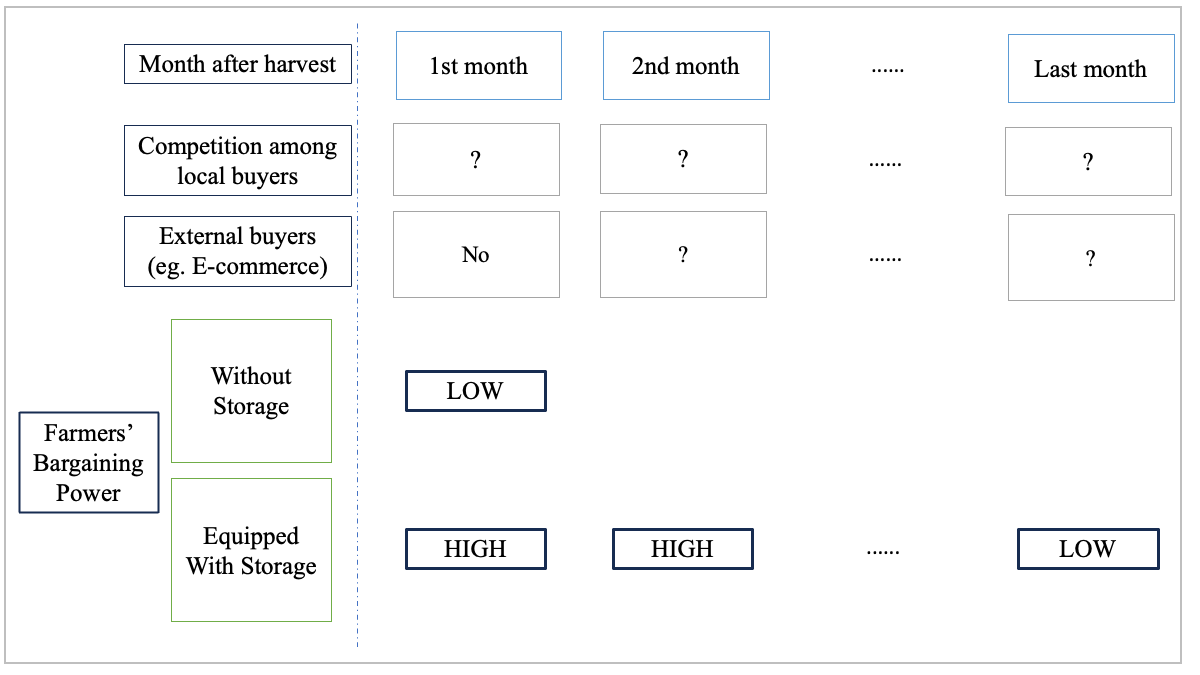
\includegraphics[width=1\textwidth]{Figures/graphic_demo.png}
\caption{Extended Marketing Opportunities from Storage Adoption}
\label{Figure: Demo}
\end{figure}

Specifically, farmers could potentially benefit from increased competition in the oligopsonistic market through two sources. Firstly, the presence of different intermediaries in the village at various times can create fluctuating levels of competition on a monthly or even weekly basis. Traders may perceive villages with greater storage as having a lower instantaneous supply of storable goods due to a smaller fraction of farmers being forced to sell. This perception leads traders to be willing to offer higher prices in these villages to secure the available supply. This allows farmers with storage options to sell their produce at the most advantageous time. Secondly, farmers with storage can tap into additional distribution channels such as e-commerce and direct selling, which differ from the conventional middlemen-dominated system. By doing so, they can introduce external participants into the oligopsonistic market at the farm gate at different time nodes. 

I develop a conceptual framework to explore how smallholder farmers adopt cold storage to bargain against the time-varying oligopsony power of middlemen. It considers a simplified dynamic two-period scenario in a developing country, where farmers sell a specific cash crop to middlemen due to high transaction costs associated with accessing larger markets. The model incorporates a storing-decision process, wherein farmers, observing farm-gate prices at harvest, decide whether to sell or store their crops. The framework shows that, absent an opportunity to observe more "draws" of the buyer-side competitive conditions, farmers would always sell during the first post-harvest period and avoid carrying costs or quality deterioration. The empirical evidence from the post-harvest decisions by small-scale apple growers in Central China further confirms the theoretical prediction. 

The outcomes of this study hold substantial implications for policymakers and farmers alike. By exploring the dynamics of time-varying oligopsony levels, the research aims to demonstrate the potential benefits of storage facilities for both producers and consumers. In a broader context, the findings suggest that embracing storage adoption could provide farmers with an effective alternative to combat anticompetitive practices like market division and avoid more intrusive measures into markets, such as governments fixing prices.

%--------------------------------------------------------%
\section{Literature Review}
    \subfile{1a_LR.tex}



%--------------------------------------------------------%
\section{Conceptual Framework}
    \subfile{1b_CF.tex}




%--------------------------------------------------------%
%--------------------------------------------------------%
    \subfile{1c_EE.tex}


%--------------------------------------------------------%
\section{Conclusion}
\noindent This chapter demonstrates that on-farm storage adoption can have a dynamic impact on the welfare of farmers facing oligopsony power, providing inter-temporal arbitrage opportunities and stronger bargaining power over time. Cold storage adoption, especially for storable crops, helps farmers overcome trading-time limitations and benefit even from temporal changes in trader competition alone. Examining storage from a market competition perspective offers a fresh approach to analyzing the influence of inventory on growers' and sellers' marketing strategies and their bargaining power.

My baseline model provides a theoretical basis for small-scale farmers' storage and marketing choices in developing countries. It focuses on farmers' intra-seasonal strategies and the storing-decision process, where farmers observe farm-gate prices at harvest and decide whether to immediately sell some, all, or none of their crops. When farmers have insufficient bargaining power at a single point in time, the adoption of storage at lower storage costs would give them inter-temporal arbitrage opportunities. 

The empirical evidence from post-harvest decisions by small-scale apple growers in Central China supports the theoretical predictions, highlighting the vulnerability of farmers to significant price cutting from middlemen in the absence of proper cold storage adoption. 

Therefore, in many developing countries, future government policies can replace or supplement the existing minimum purchase price and direct cash transfers by subsidizing farmers' investment in storage infrastructure. Instead of intervening directly into markets, by encouraging the use of on-farm technology in a broad sense to sell their harvest at an optimal time, the government can empower weak farmers to gain stronger bargaining power against middlemen and hence benefit both consumers and growers in agricultural industry supply chains.

This chapter's application extends beyond the fresh apple industry to various settings. Cold storage and inventory play a crucial role in transactions, commonly seen as tools to help sellers take advantage of business cycle fluctuations. However, the competitive dynamics among buyers can vary over time, even without changes in demand or supply elsewhere in the industry chain. By examining storage from a market competition perspective, this model offers a fresh approach to analyzing the influence of inventory on growers' and sellers' marketing strategies and their bargaining powers in agricultural commodity industries.












\newpage
\bibliography{reference.bib}

%--------------------------------------------------------%
\appendix

\newpage
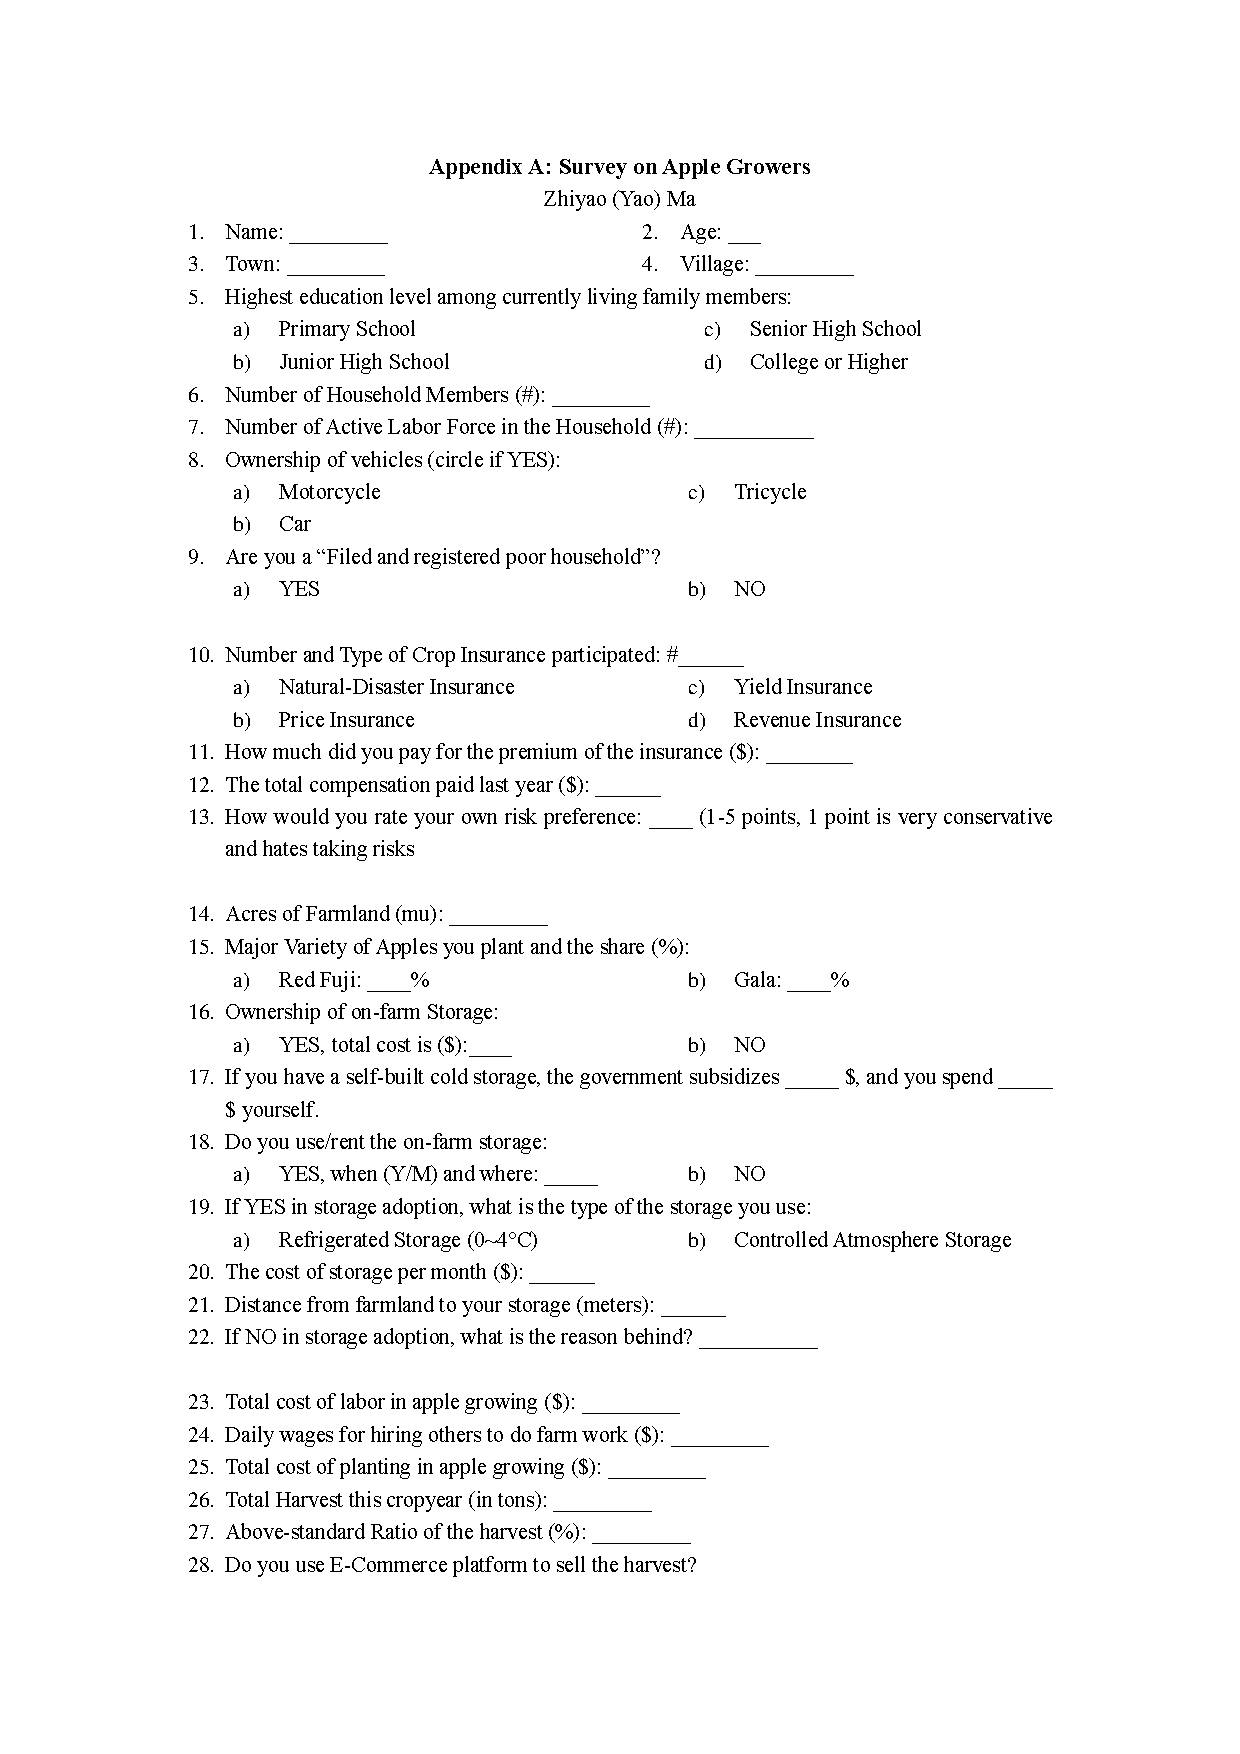
\includepdf[pages=-]{Appendix/farmers_survey.pdf}

\end{document}